% Tento soubor nahraďte vlastním souborem s obsahem práce.
%=========================================================================
% Autoři: Michal Bidlo, Bohuslav Křena, Jaroslav Dytrych, Petr Veigend a Adam Herout 2019

% Pro kompilaci po částech (viz projekt.tex), nutno odkomentovat a upravit
%\documentclass[../projekt.tex]{subfiles}
%\begin{document}


\newcommand{\highlight}[1]{\colorbox{purple}{\color{white}#1}}
\newcommand{\todoimage}[2]{
    \begin{figure}[H]
        \centering
        
\includegraphics[#1]{obrazky-figures/placeholder.pdf}
        \caption{\textbf{#2} \todo{popisek}}
    \end{figure}
}

\renewcommand{\dummyShortText}[1][1]{}
\renewcommand{\dummyText}[1][1]{}
\renewcommand{\DummyText}{}

%\renewcommand{\todoimage}[2]{}


\newcommand{\pdfcode}[3]{

    \noindent\begin{minipage}{\linewidth}
        \hfill
        \lstinputlisting[style=myPDF, caption={#2}, label=#3]{#1}
    \end{minipage}

}


%TODO: všechny odkazy na knihy rozepsat "z knihy [5]" -> "z knihy Pejsek a Kočička [5]"
%TODO: k odkazům přidat footnote na přesné nalezení + třeba dopsat v jaké kapitole / na jaké stránce
%TODO: odkazy v textu na výpisy


%*********************************************************************************
%                                    1 ÚVOD
%*********************************************************************************
\chapter{Úvod}

Pro úspěšné dokončení vysokoškolského studia musí student napsat několik desítek
stran textu zvaného závěrečná práce. Tato technická zpráva by měla být před jejím
zveřejněním několikrát překontrolována, ale ve většině případů se nenaleznou
všechny vyskytované chyby. Při velké koncentraci chyb se může výsledná práce zdát
\uv{odfláklá} a~může tak být sníženo její ohodnocení \highlight{případně přímo zamítnuta}.

V~současné době existuje několik nástrojů pro kontrolu textu. Tyto nástroje se
však převážně zaměřují na gramatické chyby a~typografické chyby tak bývají často
přehlíženy. Při správné volbě textového procesoru jsou některé chyby automaticky
při psaní opravovány, ale opět na to není žádná aplikace zaměřena.

Cílem této práce je zkoumáním zveřejněných diplomových prací nalézt, které chyby
se v~nich často vyskytují. Dalším krokem bylo navrhnout a~vytvořit lehce
dostupnou aplikaci, která nalezne tyto (převážně typografické) chyby a~označí
je přímo uvnitř poskytnutého PDF souboru. Tato aplikace by měla být dostupná bez
nutnosti instalování a~měla by být co nejvíce intuitivní.

V~kapitole \dots \todo{TODO: popis kapitol}


\dummyText

\dummyText[2]

\dummyShortText[15]

%*********************************************************************************




%*********************************************************************************
%                                2 ČASTÉ CHYBY
%*********************************************************************************
\chapter{Typografie a~často vyskytované chyby v~diplomových pracích} \label{frequent_mistakes}
U~psaní textu se autor musí řídit nejen gramatickými, ale i~typografickými
pravidly. Toto platí především při psaní odborné práce. Větší množství chyb
v~textu práce může mít za následek to, že i~kvalitně odvedená praktická realizace
práce se bude zdát neuspokojivá.

Chyby mohou být způsobeny z~nepozornosti, anebo z~neznalosti, přičemž druhá možnost
je pro autora textu horší, jelikož i~po několikátém přečtení nemusí pisatel vůbec
poznat, že se jedná o~chybu. Správnou volbou textového editoru si tvůrce textu
může usnadnit hledání některých chyb. Několik dnešních textových procesorů poskytuje
alespoň částečnou kontrolu pravopisu, nicméně tato kontrola umí ve spoustě případů
upozornit převážně jen na překlepy. Významové chyby, jako je například záměna slov
\emph{tip, typ} nebo \emph{autorizace, autentizace}, bývají často touto
automatickou kontrolou zanedbávány. Další části této kapitoly popisují několik
chyb, které lze nalézt v~mnoha diplomových pracích a~dále uvádějí, jak se těmto
chybám vyhnout.


%#######################    2.1 Rychlokurz typografie    #######################
\section{Rychlokurz typografie}
\todo{TODO: text}
\DummyText


%#######################    2.2 Přetečení objektů za okraj stránky    #######################
\section{Přetečení objektů za okraj stránky}
Přetečení textu za okraj se nejčastěji vyskytuje, když student píše svou diplomovou
práci s~pomocí jazyka {\LaTeX}. Obvykle je to způsobeno tím, že program nedokáže
automaticky zalomit slovo na konci řádku, jak je ukázáno na
obrázku~\ref{pic_overflow}. Toto lze opravit napověděním možného
zalomení nebo přeformulováním věty, kde se daná chyba vyskytuje.
Další typ této chyby je přetečení obrázku za okraj,
který se nestává tak často, ale lze jej udělat v~několika textových editorech.

\begin{figure}[H]
    \label{pic_overflow}
    \centering
    %
\includegraphics[width=\linewidth,height=1.7in]{obrazky-figures/placeholder.pdf}
    
\includegraphics{obrazky-figures/placeholder.pdf}
    \caption{\textbf{Ukázka přetečení za okraj.} \todo{popisek + přetečení obrázku}}
\end{figure}


%#######################    2.3 Spojovník x pomlčka    #######################
\section{Chybné použití spojovníku}
Nesprávné používání spojovníku je chyba, která se vyskytuje nejen v~diplomových
pracích. Spojovník (-) je graficky velmi podobný pomlčce (--), ale významově
se značně liší. Pravidla pro psaní těchto znaků, uvedena v~internetové příručce
Ústavu pro jazyk český~\cite{Ustav_pro_jazyk_cesky},
říkají, že spojovník se píše bez mezer mezi výrazy, které spojuje. Výjimkou
je, naznačuje-li spojovník neúplné slovo. Obecně se tedy v~češtině tento znak
užívá tehdy, \highlight{chce-li autor vyjádřit}, že jím spojené výrazy tvoří těsný významový
celek. Pomlčka se oproti spojovníku využívá pro oddělování částí projevu,
vyjádření rozsahu, vztahu nebo vyznačení přestávky v~řeči, pro uvození
přímé řeči a~pro vyjádření celého čísla při psaní peněžních částek.
Odděluje se z~obou stran mezerami. Komplikovanější situace nastane pouze
tehdy, když je toto znaménko použito ve funkci výrazů a, až, od, do nebo proti.
Spojovník (-) i~pomlčka (--) bývají často zaměňovány se znaménkem minus ($-$),
to však má též své grafické i~významové odlišnosti.
V~knize~\cite{Pruvodce_tvorbou_dokumentu} je vysvětleno, že znak minus má stejnou
šíři i~umístění jako znak plus. Znak minus se používá ve dvou významech, a to
pro označení záporné hodnoty, nebo pro označení operace odčítání. Sazba se v~obou
případech liší: pro označení záporné hodnoty se znak minus a~následující
operand píše bez mezery, pro psaní minus jako odčítání se však mezera uvádí
z~obou stran tohoto znaménka. Internetová příručka Ústavu pro jazyk
český~\cite{Ustav_pro_jazyk_cesky} však uvádí, že je v~korespondenci dovoleno
znak minus ($-$) nahradit pomlčkou (--).

Podle článku~\cite{Zaklady_typografie:Slezakova} se tato chyba (naznačena na
obrázku~\ref{TODO:}) vyskytuje v~textu kvůli absenci znaku pomlčky na klávesnici.
Místo znaku pomlčky, který je při psaní textu pravděpodobně potřebný častěji,
se na klávesnici vyskytuje právě znak spojovníku. I~když nyní už spousta
textových editorů dokáže automaticky nahradit spojovník za pomlčku, tato náhrada
nemusí být stoprocentní. V~programu {\LaTeX} se spojovník zapíše přímo
z~klávesnice jako \verb|-|,
pomlčku je možno zapsat pomocí dvou spojovníků \verb|--| a~znaménko minus je
zapsáno jako spojovník v~matematickém prostředí \verb|$-$| nebo též \verb|$$-$$|.

\todoimage{width=\linewidth,height=1.7in}{Ukázka chybně použitého spojovníku.}


%#######################    2.4 Chybějící popis kapitoly    #######################
\section{Chybějící popis kapitoly}

I~když je kapitola rozdělena na několik podkapitol, musí i~samotná kapitola
obsahovat úvod do této kapitoly. Blog~\cite{Leany_blog} vysvětluje, že pokud není uveden
popis mezi kapitolou a~její podkapitolou, působí poté práce nedopracovaně. Tuto
skutečnost lze vidět i~na ukázce v~obrázku~\ref{TODO:}. V~tomto místě
se hodí napsat 1--2 odstavce, kde bude vysvětlené o~čem daná kapitola je a~co se
v~ní čtenář dozví.
\todoimage{width=\linewidth,height=1.7in}{Ukázka chybějícího textu.}


%#######################    2.5 Nadpisy třetí a větší úrovně v obsahu    #######################
\section{Nadpisy třetí a~větší úrovně v~obsahu}
V~diplomové práci není vhodné v~obsahu uvádět nadpisy třetí či větší úrovně.
Jak je vidět na obrázku~\ref{TODO:}, obsah je poté nepřehledný a~zbytečně
dlouhý. Samotná třetí úroveň nadpisů je velmi podrobná, ale v~diplomové práci
ji lze použít v~případě, když bude nečíslovaná. V~programu {\LaTeX} tohoto lze dosáhnout
příkazem \verb|\subsection*{}|. Nadpisy čtvrté a~větší úrovně už by se v~diplomové
práci neměly vůbec vyskytovat.

\todoimage{width=\linewidth,height=1.7in}{Ukázka obsahu s~nadpisy 3 a~více úrovně.}


%#######################    2.6 Absence vektorové grafiky    #######################
\section{Absence vektorové grafiky} \label{vector_graphic}
Při vkládání obrázku do textu se autor musí zabývat několika otázkami a~jedna
z~nich je určitě jeho kvalita. Pokud má obrázek moc malé rozlišení
nevypadá v~odborné práci dobře. I~přesto, že se obrázek na displeji zdá
dostatečně kvalitní, při tisku může být daný obrázek \uv{rozkostičkovaný}.
Toto nevhodné použití lze vidět i~na obrázku~\ref{TODO:}.
Tento problém kvalitního rozlišení nám může vyřešit použití vektorového obrázku.
Podle knihy~\cite{Pruvodce_tvorbou_dokumentu} je zásadní výhodou vektorového
obrázku jeho uložení, díky kterému si obrázek ponechá vysokou kvalitu i~v~různém
zvětšení. Ale použití vektorové grafiky není vždy vhodné a~v~některých případech
není ani možné. V~knize je proto uvedeno doporučení použít vektorovou grafiku
(formáty SVG, EPS a~PDF) na schémata a~loga, rastrovou grafiku formátu JPG pro
fotografie a~pro ostatní rastrovou grafiku použít formát PNG.

\todoimage{width=\linewidth,height=1.7in}{Ukázka rastrového a~vektorového obrázku.}


%#######################    2.7 Nepoužívání pevné mezery    #######################
\section{Nepoužívání pevné mezery}
Jako spousta jiných věcí i~psaní mezer má svá pravidla. Jak zmiňuje
článek~\cite{Ctenar_12_2015}, i~v~něčem tak samozřejmém, jako je psaní pouhé
mezery se často chybuje: mezera se musí psát za tečkou (nebo též čárkou), ne před
ní a~píše se vždy jen jedna, data se píšou ve formátu \emph{d.~m. yyyy}
a~čísla se oddělují mezerou po tisících (s~výjimkou letopočtu). Při psaní se může
stát, že mezera spojující znaky nebo čísla, vyjde na konec řádku a~tyto znaky
by se rozdělily. Tento případ lze pozorovat i~na obrázku~\ref{TODO:}.
Pro zamezení takových případů existuje právě pevná (nebo též nedělitelná)
mezera.

Pevná mezera se zobrazí stejně jako normální mezera, ale na rozdíl od normální
mezery, spojí dohromady příslušné znaky a~zablokuje jejich rozdělení na konci
řádku. Podle pravidel internetové jazykové příručky~\cite{Ustav_pro_jazyk_cesky}
se má pevná mezera použít v~těchto případech (převzato a~upraveno):
\begin{itemize}
    \item ve spojení neslabičných předložek \emph{k, s, v, z} s~následujícím
    slovem, např. \emph{v~obrázku, z~funkce},
    \item ve spojení slabičných předložek \emph{o, u} a~spojek \emph{a, i}
    s~následujícím výrazem, např. \emph{o~kapitole, a~to},
    \item členění čísel, např. $\mathit{2\,301\,000}$, $\mathit{3,\!141\,592\,65}$,
    \item mezi číslem a~značkou, např. \emph{25~\%, \copyright~2008},
    \item mezi číslem a~zkratkou počítaného předmětu nebo písmennou značkou
    jednotek a~měn, např. \emph{24~hod., 100\,m, 3\,000~Kč, 500~¥},
    \item mezi číslem a~názvem počítaného jevu, např. \emph{obrázek~5, 12~metrů,
    I.~patro},
    \item v~kalendářních datech mezi dnem a~měsícem, rok však lze oddělit, např.
    \emph{3.~5. 2000, 26.~dubna 2023}
    \item v~měřítkách map, plánů a~výkresů, v~poměrech nebo při naznačení dělení,
    např. \emph{4~:~7, 1~:~10~000}, $\mathit{12:2=6}$,
    \item v~telefonních, faxových a~jiných číslech členěných mezerou, např. 
    \emph{+420~603~999~226},
    \item ve složených zkratkách (v~případě nutnosti se doporučuje dělit podle
    dílčích celků), v~ustálených spojeních a~v~různých kódech, např.
    \emph{s.~r.~o., m~n.~m., ISO~690},
    \item mezi zkratkami typu \emph{tj., tzv., tzn.} a~výrazem, který za nimi
    bezprostředně následuje, např. \emph{tzv.~pipeline},
    \item mezi zkratkami rodných jmen a~příjmeními, např. \emph{T.\,Milet},
    \item mezi zkratkou titulu nebo hodnosti uváděnou před osobním jménem, např.
    \emph{p.~Macková, Ing.~Novák}.
\end{itemize}

Zapsání pevné mezery závisí na použitém textovém editoru. I~když spousta z~nich
již umí tuto pevnou mezeru automaticky doplnit, nemusí mít tato automatizace
stoprocentní úspěšnost. V~programu {\LaTeX} se pevná mezera zapíše znakem tildy
(\texttildelow) a~v~editoru WORD se zapíše pomocí kombinace kláves
\emph{Ctrl Shift mezera}.

\todoimage{width=\linewidth,height=1.7in}{Ukázka.}

%#######################    2.8 Použití nesprávných uvozovek    #######################
% \section{Použití nesprávných uvozovek}
% \dummyText
% \todoimage{width=\linewidth,height=1.7in}{Ukázka.}

% %#######################    2.9 Špatný odkaz na referenci    #######################
% \section{Špatný odkaz na referenci}
% \dummyText
% \todoimage{width=\linewidth,height=1.7in}{Ukázka.}


%*********************************************************************************




%*********************************************************************************
%                               3 ANOTACE V PDF
%*********************************************************************************
\chapter{PDF soubor}

\todo{TODO: úvod do kapitoly}
\dummyText



%#######################    3.1 Formát PDF    #######################
\section{Formát PDF} \label{format_PDF}
Většina uživatelů, kteří zachází s~PDF soubory nepotřebují znát vnitřní složení
PDF dokumentů. Spousta programů a~knihoven, pro vytváření či úpravu PDF dokumentu
dokáže při práci s~tímto souborem dostatečně odstínit od syntaxe PDF formátu.
Avšak pro pokročilejší práci s~PDF dokumenty není na obtíž si zjistit pár
základních informací o~uložení dat v~tomto formátu.
PDF dokument má podobu textového souboru a~na jeho pochopení jsou v~této sekci
vysvětleny jeho 4 základní stavební bloky. Tato sekce čerpá informace ze
standardu PDF~32000-1~\cite{PDF32000-1:2008}.


%---------- 3.1.1 Objekty ----------
\subsection*{Objekty}
Objekty jsou jedny ze základních stavebních bloků PDF dokumentu. PDF rozeznává
osm typů objektů:
\begin{itemize}
    \item \textbf{Boolean objekt} -- Tyto objekty reprezentují logickou hodnotu.
    Můžou nabýt dvou hodnot, které jsou označeny klíčovými slovy \texttt{true}
    a~\texttt{false}.
    
    \item \textbf{Číselný objekt} -- Obsahovaná číselná hodnota může být celé,
    nebo reálné číslo. U~zápisu reálných čísel se používá desetinná tečka,
    například \texttt{-3.62}, \texttt{.054}, \texttt{+238.45}. Celá čísla můžou
    být například \texttt{500}, \texttt{+3}, \texttt{-21}.
    
    \item \textbf{Řetězcový objekt (string)} -- Řetězec lze zapsat dvěma způsoby,
    a~to jako klasický řetězec, nebo jako řetězec v~hexadecimální podobě. Klasický
    řetězec je zapsán jako posloupnost znaků uzavřená v~kulatých závorkách,
    například \texttt{(Toto je string)}. V~tomto typu řetězce je možné používat
    escape sekvence začínající zpětným lomítkem. Řetězec psaný v~hexadecimální
    podobě lze zapsat jako posloupnost hexadecimálních číslic uzavřenou mezi znaky
    menší než a~větší než, například \texttt{<48656c6c6f>}, \texttt{<776F726C64>}.
    Každá dvojice hexadecimálních číslic tvoří jeden znak zakódovaný v~ASCII
    podobě.
    
    \item \textbf{Jmenný objekt} -- Objekt jména je sekvence znaků. Znaky, které
    se mohou použít ve jménu jsou takové, které zapadají do rozmezí mezi znakem
    vykřičníku (!) a~znakem tildy (\texttildelow). Ostatní znaky se mohou zapsat
    jako hexadecimální hodnota požadovaného znaku, kterou předchází znak mřížky
    (\#). Jméno musí začínat lomítkem, které se nebere jako jeho součást. Zapsané
    jméno může být například \texttt{/Name}, \texttt{/1.6*xyz}, \texttt{/C\#23}.
    
    \item \textbf{Objekt pole} -- Objekt typu pole je kolekce, která obsahuje
    objekty. Tyto objekty nemusí být stejného typu -- heterogenní pole.
    Zapisuje se jako prvky pole, které jsou odděleny bílým znakem, uzavřené
    v~hranatých závorkách. Prvkem pole může být objekt pole. Validní pole je
    například \texttt{[(string) -25 [2.75 /Name] true]}.
    
    \item \textbf{Slovníkový objekt} -- Slovník je kolekce, jejíž prvky jsou
    dvojice objektů. První prvek z~této dvojice se nazývá \emph{klíč} a~vždy to 
    musí být objekt typu jméno. Ve slovníku nesmí existovat více záznamů se
    stejným klíčem. Druhý prvek ze dvojice se nazývá \emph{hodnota}.
    Tento prvek může být objekt jakéhokoli typu. Slovník je uvozen dvojitým znakem
    menší než a~dvojitým znakem větší než, například
    \texttt{<</Key1 2.6 /Key2 /Value2>>}.

    \item \textbf{Objekt datového toku (stream)} -- Stream je sekvence bajtů, 
    která má neomezenou délku. Používá se především pro ukládání velkého množství
    dat, což je například obrázek. Tento objekt se zapisuje jako slovník, za nímž
    následuje klíčové slovo \texttt{stream}, po kterém se musí vyskytovat konec
    řádku. Následují bajty datového toku, které jsou ukončeny koncem řádku
    a~klíčovým slovem \texttt{endstream}. Vyskytovaný slovník nesmí být uveden
    nepřímým odkazem a~musí se v~něm uvádět délka datového toku v~bajtech, pod
    klíčem \texttt{Length}. Každý objekt datového toku musí být zároveň nepřímým
    objektem (vysvětleno později v~této sekci). Validní objekt datového toku je
    například uveden ve výpise~\ref{code_stream}:
    \pdfcode{code_examples/pdf_code/stream_objects.txt}{TODO:}{code_stream}

    \item \textbf{Null objekt} -- Null objekt je speciální objekt, který nabývá
    pouze hodnoty \texttt{null}.
\end{itemize}

Každému objektu se může přiřadit jednoznačný identifikátor, takový objekt se poté
nazývá \textbf{nepřímý objekt}. Na nepřímý objekt potom může být odkazováno
z~jiného objektu, čehož je často využíváno například ve slovníku, kde je uveden
klíč a~hodnota je nepřímý odkaz na objekt. Identifikátor nepřímého objektu má dvě
části. První část je kladné celé číslo, kterému se říká \emph{číslo objektu}.
Druhou částí je tzv. \emph{číslo generace}, které je pro nově generovaný dokument
0. Toto číslo musí být vždy nezáporné celé číslo. Nepřímý objekt se zapíše jako
číslo objektu, poté bílý znak a~číslo generace. Následuje samotný objekt uzavřen
mezi klíčovými slovy \texttt{obj} a~\texttt{endobj}. Validní nepřímý objekt je
například:
\pdfcode{code_examples/pdf_code/indirect_object.txt}{TODO:}{code_indirect_object}
\noindent Nepřímý objekt lze referencovat pomocí \emph{nepřímého odkazu}.
Nepřímý odkaz se zapíše číslem objektu, číslem generace a~klíčovým slovem
\texttt{R}, oddělené bílými znaky. Odkaz na výše uvedený nepřímý objet se zapíše
jako \texttt{7 0 R}.


%---------- 3.1.2 Struktura souboru ----------
\subsection*{Struktura souboru}
Tato část popisuje, jak jsou výše popsané objekty uložené v~PDF dokumentu.
Též popisuje, jak je k~nim přistupováno a~jak jsou aktualizovány.
PDF soubor se je rozdělen do 4~částí: 
\begin{itemize}
    \item \textbf{Hlavička} -- Hlavička se vždy vyskytuje na prvním řádku souboru.
    Má tvar komentáře, přesněji \texttt{\%PDF–} a~bezprostředně za tím následuje
    číslo PDF verze, například \texttt{\%PDF–1.7}.
    
    \item \textbf{Tělo} -- Tělo se skládá z~posloupnosti nepřímých objektů. Tyto 
    nepřímé objekty popisují vzhled celého dokumentu (stránky, fonty, obrázky,
    \ldots).
    
    \item \textbf{Tabulka křížových odkazů} -- Tabulka křížových odkazů se používá
    při přístupu k~nepřímým objektům. Tato tabulka obsahuje informaci o~umístění
    každého nepřímého objektu. Tabulka se skládá z~jedné nebo více \emph{sekcí
    křížových odkazů}, která musí začínat řádkem s~klíčovým slovem \texttt{xref}.
    Každá sekce může být rozdělena na několik \emph{podsekcí křížových odkazů}.
    Tyto podsekce vždy začínají řádkem, na kterém se vyskytují dvě čísla. První
    číslo označuje první objekt v~záznamu podsekce a~druhé číslo značí, kolik
    takových záznamů se v~dané podsekci vyskytuje. Pod tímto řádkem se nachází
    samotné záznamy o~nepřímých objektech. Záznam o~využívaném nepřímém objektu
    má tvar \emph{nnnnnnnnnn ggggg \texttt{n}} a~je zakončen koncem řádku.
    Desetimístné číslo \emph{nnnnnnnnnn} označuje offset bajtů od začátku
    dokumentu, po začátek nepřímého objektu. Pětimístné číslo \emph{ggggg} je
    číslo generace. Jedna sekce křížových odkazů, rozdělena na 2~podsekce, celkově
    obsahující 3~záznamy může vypadat například:
    \pdfcode{code_examples/pdf_code/cross_reference_table.txt}{TODO:}{code_cross_reference_table}
    \todo{od verze 1.5 může být ve streamu}
    
    \item \textbf{Patička} -- Patička umožňuje rychlé nalezení tabulky křížových
    odkazů a~jiných speciálních objektů. Proto obecně platí, že by se měl PDF
    soubor číst od konce, kde se vykytuje právě patička. Patička začíná klíčovým
    slovem \texttt{trailer}, za ním následuje slovník patičky a~klíčové slovo
    \texttt{startxref}. Na novém řádku se poté vykytuje číslo, uvádějící počet
    bajtů offsetu od začátku souboru po začátek tabulky křížových odkazů. Jako
    poslední se na samostatném řádku musí objevit výraz \texttt{\%\%EOF}.
    V~celém souboru se může vyskytovat více patiček, to je způsobeno aktualizováním
    daného PDF dokumentu. Na posledním řádku souboru se vždy musí vyskytovat
    výraz \texttt{\%\%EOF}. Patička může vypadat následovně:
    \pdfcode{code_examples/pdf_code/trailer.txt}{TODO:}{code_trailer}
    \todo{od verze 1.5 může být slovník ve streamu}

\end{itemize}

\todoimage{width=\linewidth,height=1.7in}{Ukázka struktury souboru + odkaz.}


%---------- 3.1.3 Struktura dokumentu ----------
\subsection*{Struktura dokumentu} \label{document_structure}
\highlight{Struktura dokumentu popisuje, jak vypadá vyobrazený dokument.}
Lze si ji představit jako hierarchii objektů vyskytujících se v~těle PDF souboru.
Některé z~důležitých částí tohoto hierarchického stromu jsou:
\begin{itemize}
    \item \textbf{Katalog dokumentu} -- Tento katalog je kořenem celého
    hierarchického stromu. Odkaz na něj lze nalézt ve slovníku patičky, pod klíčem
    \texttt{Root}. Tento katalog obsahuje odkazy na objekty specifikující vzhled
    dokumentu. Objekt katalogu je slovník, ve kterém se musí vyskytovat klíč
    \texttt{Type}, ke kterému je přiřazena hodnota \texttt{/Catalog}. Dalším
    povinným prvkem katalogového slovníku je klíč \texttt{Pages}, jehož hodnota je
    nepřímý odkaz na kořenový objekt stromu stránek. Objekt katalogu dokumentu
    může být například:
    \pdfcode{code_examples/pdf_code/document_catalog.txt}{TODO:}{code_documet_catalog}

    \item \textbf{Strom stránek} -- Strom stránek určuje pořadí zobrazení stránek.
    Listové uzly tohoto stromu jsou typu \emph{objektu stránky}, které mají jiný
    tvar než ostatní uzly tohoto stromu. Uzly stromu stránek jsou typu slovníku,
    ve kterém se musí vyskytovat klíče \texttt{Type}, \texttt{Kids},
    \texttt{Count} a~\texttt{Parent}, jenž není povinný v~kořenovém uzlu.
    Hodnota klíče \texttt{Type} musí v~uzlu stromu stránek být \texttt{/Pages}.
    Ke klíči \texttt{Kids} musí být přiřazena hodnota typu pole, které obsahuje
    nepřímé odkazy na uzly stromu stránek, nebo na objekty stránek. Hodnota klíče
    \texttt{Count} je počet listových uzlů, které jsou potomkem tohoto uzlu. Ke
    klíči \texttt{Parent} je přiřazena hodnota nepřímého odkazu přímého předchůdce
    tohoto uzlu. Uzel stromu stránek může být například:
    \pdfcode{code_examples/pdf_code/page_tree.txt}{TODO:}{code_page_tree}

    \item \textbf{Objekt stránky} -- Objekt stránky je typ listového uzlu stromu
    stránek. Tento uzel má tvar slovníku, ve kterém se musí vyskytovat klíč
    \texttt{Type} s~hodnotou \texttt{/Page}. Dalším povinným záznamem tohoto
    slovníku je klíč \texttt{Parent}, jehož hodnota je nepřímý odkaz na přímého
    předchůdce tohoto listového uzlu stromu stránek. Mezi jiné důležité záznamy
    patří záznamy s~klíčem \texttt{MediaBox}, \texttt{Resources} \highlight{(popsáno dále
    v~této kapitole)}, \texttt{Rotate},
    \texttt{Contents} \highlight{(popsáno dále v~této kapitole)}, \texttt{Annots} aj.
    Jednoduchý objekt stránky může vypadat následovně:
    \pdfcode{code_examples/pdf_code/page_object.txt}{TODO:}{code_page_object}
\end{itemize}


%---------- 3.1.4 Content streams ----------
\subsection*{Content streams} \label{content_streams}
Content stream obsahuje popis vzhledu PDF stránky pomocí instrukcí na její
vykreslení. Tyto instrukce jsou zapsány pomocí PDF objektů, ale na rozdíl od
PDF dokumentu jsou tyto instrukce seřazené a~vykonávají se podle jejich
posloupnosti. \emph{Operand} takové instrukce musí být přímý objekt, který 
nesmí být typu datového toku. Operand může být typ slovník pouze při použití
speciálních operací. \emph{Operátor} instrukce určuje, která akce se provede.
Operátory jsou klíčová slova typu jmenného objektu, kde na rozdíl od PDF dokumentu
se operátory píšou bez počátečního lomítka. Content stream používá pro zapsání
instrukcí postfixovou notaci, tedy nejdříve jsou uvedeny všechny operandy instrukce
a~poté je uveden její operátor.


%---------- 3.1.5 Resources ----------
\subsection*{Resources} \label{resources}
Resources specifikují a~pojmenovávají používané externí objekty z~content streams.
V~content streams se nesmí používat nepřímé odkazy, proto je možné pojmenovat
jednotlivé používané objekty a~definovat je tak jako \emph{named resources}.
Tyto jména lze používat pouze uvnitř content streams a~mimo ně nejsou v~PDF
dokumentu validní. Named resources se používají například pro obrázky a~fonty,
které jsou použity na dané stránce. Objekt pro resources je typu slovníku, který
má několik definovaných klíčů, které je možné použít, např. \texttt{ColorSpace}, 
\texttt{XObject}, \texttt{Font}, \texttt{ProcSet} a~další. Slovník pro resources,
který obsahuje font pod jménem \texttt{F5} a~dva externí objekty pojmenované jako
\texttt{Im1} a~\texttt{Im2}, může vypadat následovně:
\pdfcode{code_examples/pdf_code/resources.txt}{TODO:}{code_resources}
\todo{F5, Im1 a Im2 správné zvýraznění? (emph vs texttt vs none)}



%#######################    3.2 Grafika v~PDF    #######################
\section{Grafika v~PDF}
Tato sekce čerpá informace ze standardu PDF~32000-1~\cite{PDF32000-1:2008}.
Grafika PDF dokumentu je popsána pomocí content streams, jenž je vysvětleno
v~kapitole~\ref{content_streams}. Operátory zde používané spadají do šesti
hlavních skupin:
\begin{itemize}
    \item \textbf{Graphics state operátory} -- Tyto operátory manipulují
    s~datovou strukturou zvanou \emph{graphics state}, která je vysvětlena později
    v~této kapitole.
    \item \textbf{Operátory pro konstrukci křivek} -- Jsou to operátory, které
    specifikují, jak bude vypadat vykreslená křivka. Spadají zde například
    operátory pro vytvoření nové cesty, přidávání zaoblení, přidávání nové části
    křivky a~uzavření tvaru.
    \item \textbf{Operátory pro vymalování křivek} -- Operátory vybarvující
    křivku nebo prostor vyhrazený takovou křivkou.
    \item \textbf{Další vykreslovací operátory} -- Tyto operátory se používají
    pro vykreslení grafických objektů, mezi které patří i~obrázky.
    \item \textbf{Textové operátory} -- Text se v~PDF vykreslí jako několik
    grafických částí, které jsou definovány fontem. Pomocí těchto operátorů
    se specifikují nastavení spojené s~textem a~též zde patří operátory pro
    vykreslení takového textu. 
    \item \textbf{Marked-content operátory} -- Tyto operátory přímo neovlivňují
    vzhled stránky, ale spojují informace a~objekty uvedené v~content streamu.
\end{itemize}


%---------- 3.2.1 Souřadnicové systémy ----------
\subsection*{Souřadnicové systémy}
PDF definuje více souřadnicových systémů, ve kterých se definují různé grafické
objekty. Převod mezi těmito souřadnicovými systémy se provádí s~pomocí
transformačních matic, které dokážou otáčet, posunovat nebo měnit měřítko
mapovaného objektu (nemění se přitom samotné data uloženého objektu, jen jak je
zobrazen uvnitř souřadnicového systému). V~PDF se transformační matice značí polem
obsahující šest číselných objektů $[a~b~c~d~e~f]$. Tato transformační matice je
vyobrazena v~rovnici~\eqref{transformation_matrix}.
\begin{equation}\label{transformation_matrix}
    M_T = 
    \begin{pmatrix}
        a & b & 0 \\
        c & d & 0 \\
        d & f & 1
    \end{pmatrix}
\end{equation}
Pokud se potřebuje provést více elementárních transformací 
(např. rotace a~posun), záleží na jejich posloupnosti provedení. Obecně
platí vzorec~\eqref{multiple_matrix_transformations}, kde $M_{T_1}$ značí matici
první provedené transformace, $M_{T_n}$ je matice poslední provedené transformace
a~$M'$ označuje matici, která kombinuje všechny tyto provedené transformace.
\begin{equation} \label{multiple_matrix_transformations}
    M' = M_{T_1} \cdot M_{T_2} \cdots M_{T_{n-1}} \cdot M_{T_n}
\end{equation}

Bod $(x, y)$ v~souřadnicovém systému se může matematicky popsat jako vektor
z~rovnice~\eqref{point}.
\begin{equation}\label{point}
    P = 
    \begin{pmatrix}
        x & y & 1
    \end{pmatrix}
\end{equation}
Transformovaný bod (souřadnice bodu po použití všech transformací) se vypočítá
pomocí vzorce~\eqref{transform_point}. $P$ v~tomto vzorci označuje původní vektor
transformovaného bodu, $P'$ je vektor tohoto bodu po transformaci a~$M'$ je matice
kombinující všechny provedené transformace.
\begin{equation} \label{transform_point}
    P' = P \cdot M'
\end{equation}

Dále jsou popsány souřadnicové systémy používané v~PDF. Vztahy mezi těmito
souřadnicovými systémy jsou vyznačeny na obrázku~\ref{coordinate_spaces}.
\begin{itemize}
    \item \textbf{Prostor zařízení (device space)} -- Tento souřadnicový systém je
    závislý na zařízení, kde se zobrazuje vytvořený PDF dokument. Je to poslední
    prostor, do kterého se promítá zobrazení PDF souboru. Zobrazovacím zařízením
    se rozumí například displej obrazovky počítače, papír v~tiskárně, plátno, na
    které promítá projektor aj.
    
    \item \textbf{Uživatelský prostor (user space)} -- Aby se zamezilo nevhodným
    účinkům při zobrazování do prostoru zařízení, definuje PDF vlastní prostor,
    který je nezávislý na zařízení. Tento souřadnicový systém se nazývá
    \emph{uživatelský prostor}. Pro každou stránku PDF dokumentu se tento
    souřadnicový systém uvede do původního stavu. V~uživatelském prostoru je bod
    $(0, 0)$ levý dolní roh, tedy x-ová souřadnice se zvyšuje směrem
    doprava a~y-ová souřadnice roste směrem nahoru. Rozlišení určeno v~jednotkách
    uživatelského prostoru nesouvisí s~rozlišením v~pixelech uvnitř prostoru
    zařízení. Převedení z~uživatelského prostoru do prostoru zařízení se provádí
    pomocí \emph{current transformation matrix (CTM)}. CTM je součástí datové
    struktury \emph{graphics state}, která je popsáná dále v~této kapitole.
    Aplikace zobrazující PDF si tuto CTM matici upraví podle vlastností výstupního
    zařízení, aby se zachovala nezávislost uživatelského prostoru na zařízení. 
    Vyobrazení tohoto jevu jde vidět na obrázku~\ref{pic_user_to_device}.

    \begin{figure}[H]
        \centering
        \label{pic_user_to_device}
        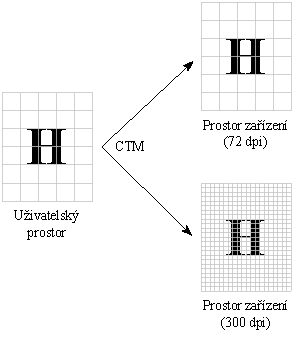
\includegraphics[width=0.5\linewidth]{obrazky-figures/user_to_device_space.pdf}
        \caption{\todo{TODO: popisek} Inspirován obrázkem ze standardu~PDF~32000-1~\cite{PDF32000-1:2008}}
    \end{figure}
    
    \item \textbf{Specializované prostory} -- PDF formát pracuje kromě
    uživatelského prostoru a~prostoru zařízení i~se specializovanými prostory.
    \begin{itemize}
        \item \emph{Textový prostor} -- V~tomto prostoru se definují souřadnice
        textu. Převod z~textového prostoru do uživatelského prostoru se provádí
        pomocí \emph{textové matice} a~několika textových parametrů vyskytujících
        se v~datové struktuře graphics state.

        \item \emph{Glyph space} -- Glyfy znaků fontu musí být definovány v~tomto
        prostoru. Z~glyph space se poté transformuje do textového prostoru.
        
        \item \emph{Obrázkový prostor} -- Všechny obrázky by měly být definovány
        v~tomto prostoru. Pro správné vykreslení obrázku na stránku se musí dočasně
        upravit CTM.

        \item \emph{Prostor formuláře} -- Formulářový \emph{XObject} (též externí
        objekt, viz dále v~této kapitole) je
        reprezentován jako content stream. Tento XObject je v~jiném content streamu
        brán jako grafický objekt. Prostor, ve kterém je tento formulář definovaný,
        se nazývá prostor formuláře.

        \item \emph{Pattern space} -- PDF formát poznává typ barvy zvaný
        \emph{pattern}. Pattern je definovaný jako content stream a~prostoru, ve
        kterém je definován se říká pattern space.
        
        \item \emph{3D prostor} -- Tento souřadnicový systém je
        trojdimenzionální a~používá se pro vložené 3D díla.
    \end{itemize}
\end{itemize}

\begin{figure}[H]
    \label{coordinate_spaces}
    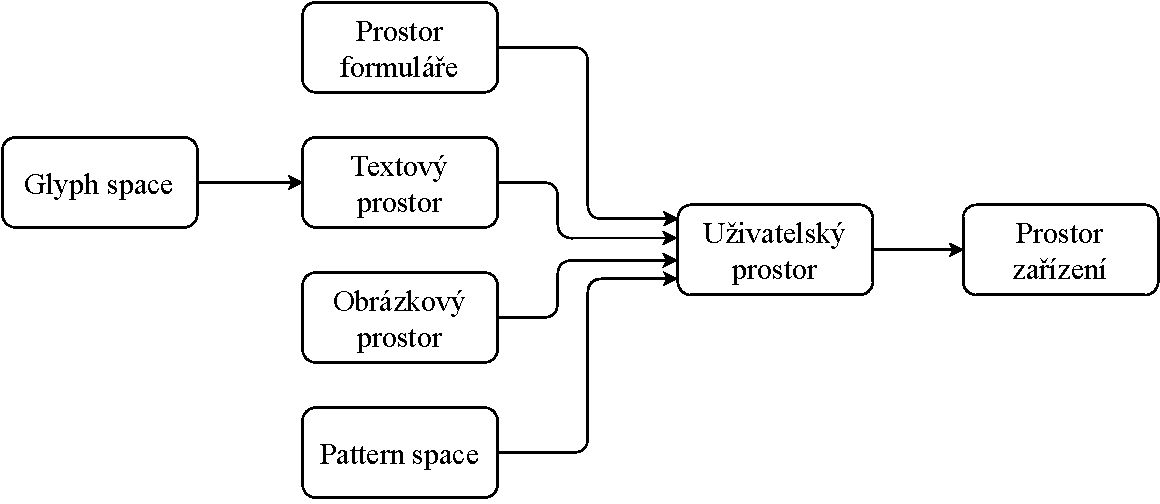
\includegraphics[width=\linewidth]{obrazky-figures/coordinate_spaces.pdf}
    \caption[Vztah mezi souřadnicovými systémy používaných uvnitř PDF]{Obrázek označuje vztah mezi souřadnicovými systémy používaných uvnitř PDF. Každá šipka představuje transformaci mezi dvěma souřadnicovými systémy. Inspirováno obrázkem ze standardu~PDF~32000-1~\cite{PDF32000-1:2008}}
\end{figure}


%---------- 3.2.2 Graphics state ----------
\subsection*{Graphics state} \label{graphics_state}
Pro zobrazení PDF dokumentu se používá datová struktura zvaná \emph{graphics state}.
Každá aplikace zobrazující PDF dokumenty musí umět udržovat tuto datovou strukturu.
Graphics state struktura v~sobě obsahuje několik parametrů, se kterými pracují
operace uvnitř content streamu (popsaný v~kapitole~\ref{content_streams}). Pro
každou stránku se na začátku musí v~graphics state struktuře nastavit výchozí
hodnoty obsahujících parametrů. Tyto parametry jsou rozděleny na dvě skupiny:
závislé na zařízení a~nezávislé na zařízení. Mezi parametry nezávislých na zařízení
patří například CTM (current transformation matrix), barva (aktuální barva
používaná při vykreslovacích operacích), stav textu (devět parametrů popisující
formát vypisovaného textu) a~tloušťka čáry. Parametry závislé na zařízení jsou
například \uv{overprint}, \uv{flatness} a~\uv{smoothness}.

Na jedné stránce se může vyskytovat několik grafických objektů, které se
vykreslují nezávisle na sobě. Pro tyto účely se používá
\emph{graphics state zásobník}, díky kterému je možné dělat lokální úpravy 
datové struktury graphics state. Tento zásobník je LIFO (last in, first out)
a~ukládá se do něj celá datová struktura graphics state. Pro uložení
se musí použít operátor \texttt{q} a~pro odebrání první položky z~vrcholu
zásobníku se musí použít operátor \texttt{Q}, kterým se obnoví posledně uložený
stav datové struktury graphics state. Uvnitř celého content streamu musí být
použit stejný počet operátorů \texttt{q} a~\texttt{Q}.

\begin{figure}[H]
    \label{pic_graphics_state}
    \centering
    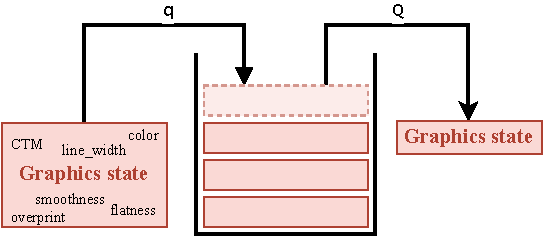
\includegraphics[width=0.7\linewidth]{obrazky-figures/graphics_state_stack.pdf}
    \caption{\todo{TODO: odkaz}}
\end{figure}

Pro úpravu parametrů uložených ve struktuře graphics state se používají uvnitř
content streamu specifické operátory. Mezi tyto operátory patří již uvedené
\texttt{q} a~\texttt{Q}, které nepoužívají žádné operandy. Další používané
operátory upravující graphics state jsou například \texttt{cm}, \texttt{w},
\texttt{i} a~jiné. K~operátoru \texttt{cm} se váže šest číselných operandů
\emph{a, b, c, d, e} a~\emph{f}. Dohromady tyto operandy specifikují matici
transformace, která bude vynásobena maticí CTM a~následně přiřazena do CTM položky
datové struktury graphics state. Operátor \texttt{w} je unární a~jeho operandem
je číslo \emph{lineWidth}, které specifikuje tloušťku kreslených čar. Unární
operátor \texttt{i} nastaví uvedený číselná operand jako \emph{flatness} parametr
struktury graphics state.



%---------- 3.2.3 Externí objekty ----------
\subsection*{Externí objekty} \label{XObject}
Externí objekt (též taky \emph{XObject}) ... \todo{TODO: obecný popis}.
Každý XObject lze vykreslit pomocí operátoru \texttt{Do} vyskytujícího se uvnitř
content streamu. K~tomuto operátoru se váže jeden operand typu jméno. Toto jméno
musí být uvedeno ve slovníku resources (viz kapitola~\ref{resources}) vázaného
na stejnou stránku jako content stream. Přesněji se toto jméno musí objevit
v~položce, která má hodnotu typu slovník, pod klíčem \texttt{XObject}. Operátor
\texttt{Do} má 3 různé chování. Toto chování závisí na hodnotě vázané ke klíči
\texttt{Subtype} uvnitř XObject slovníku, na který se odkazuje operand tohoto
příkazu. Hodnoty klíče \texttt{Subtype} a~k nim vázané chování příkazu
\texttt{Do} jsou:
\begin{itemize}
    \item \texttt{/Image} -- Tyto externí objekty mají ve slovníkové části své
    definice dodatečné prvky. Prvky s~klíčem \texttt{Width} a~\texttt{Height}
    jsou v~těchto objektech povinné. Tyto prvky můžou ovlivnit jak bude
    vykreslený obrázek vypadat, ale podle aktuálního nastavení stránky můžou mít
    omezené možnosti. \todo{Do}
    
    \item \texttt{/Form} -- Takzvaný \emph{Form XObject} je takový, který ve svém
    datovém toku obsahuje content stream (popsán v~sekci~\ref{content_streams}).
    Form XObject může být vykreslen několikrát a~to na různých souřadnicích.
    Ve slovníkové části tohoto objektu musí být pro tento typ uvedena hodnota
    pro klíč \texttt{BBox}. Tato hodnota jsou souřadnice daného externího objektu
    v~prostoru formuláře. Pro transformaci mezi formulářovým prostorem a~user
    space se uvádí použitá transformační matice jako hodnota pro klíč
    \texttt{Matrix}. Pokud tato matice není uvedena, použije se místo ní
    jednotková matice. Pro vykreslení se tohoto objektu se musí použít operátor
    \texttt{Do} a~při tom se provedou následující kroky (převzato ze standardu
    PDF~\cite{PDF32000-1:2008}):
    \begin{enumerate}
        \item Uloží se aktuální stav datové struktury graphics state, stejně
        jako kdyby byl použit operátor \texttt{q}.
        \item Vynásobí se matice ze slovníkového prvku \texttt{Matrix} a~matice
        CTM z~datové struktury graphics state.
        \item \texttt{BBox} \todo{clips}
        \item Vykreslí obsahované  grafické objekty podle instrukcí uvnitř content
        streamu definovaného objektem form XObject.
        \item Obnoví původní stav struktury graphics state (jako použití operátoru
        \texttt{Q}).
    \end{enumerate}
    
    \item \texttt{/PS} -- Takzvaný \emph{PostScript XObject} je využíván pouze
    pokud bude daný PDF dokument zpracován zařízením používající jazyk PostScript.
    Při zobrazení v~jiných zařízeních bude tento objekt ignorován. Aplikace
    zpracovávající PDF dokumenty nemají nutnost zpracování těchto objektů
    podporovat.
\end{itemize}


%#######################    3.3 Reprezentace anotací v PDF souboru    #######################
\section{Reprezentace anotací v~PDF souboru} \label{PDF_annotations}
Anotace spojují objekty (zvuk, video, text, \dots) s~pozicí na PDF stránce.
Uživatel může s~anotacemi interagovat pomocí myši a~klávesnice.
\todo{\texttt{Annotations} klíč ve slovníku stránky (viz
sekce~\ref{document_structure})} PDF dokumenty podporují několik typů anotací, 
například:
\begin{itemize}
    \item \textbf{Text} -- Tyto anotace imitují nalepovací papírky. Jsou
    zobrazeny jako ikona umístěna na určitých souřadnicích a~po interakci s~myší
    se zobrazí vyskakovací okénko s~textem této anotace. Tato anotace ignoruje
    rotaci a~změnu měřítka stránky. Ve slovníku této anotace se můžou navíc
    objevit záznamy s~klíčem \texttt{Subtype} (tento prvek je povinný a~pro tento
    typ anotace musí mít hodnotu \texttt{/Text}), \texttt{Open}, \texttt{Name},
    \texttt{State} a~\texttt{StateModel}. Příklad textové anotace lze vidět ve
    výpisu~\ref{code_text_annotation}:
    \pdfcode{code_examples/pdf_code/text_annotation.txt}{
    Anotace typu \emph{Text}, která se zobrazí jako ikona
    \emph{Note}. Po interakci s~myší se zobrazí vyskakovací okénko
    s~textem \uv{This is text annotation.}}{code_text_annotation}

    \item \textbf{Odkaz} -- Anotace odkazu slouží jako hypertextový
    odkaz na místo v~daném dokumentu nebo jako akce, která se má
    provést po jejím stisknutí. Ve slovníku takové anotace musí
    existovat povinný záznam s~klíčem \texttt{Subtype} mít hodnotu
    \texttt{/Link}. Další možné záznamy mohou být \texttt{A},
    \texttt{Dest}, \texttt{H}, \texttt{PA}, \texttt{QuadPoints}
    a~\texttt{BS}. Validní anotace odkazu je uvedena ve
    výpisu~\ref{code_link_annotation}:
    \pdfcode{code_examples/pdf_code/link_annotation.txt}{
    Anotace typu \emph{Link}, která odkazuje na místo uvnitř
    stejného dokumentu.
    }{code_link_annotation}
    
    \item \textbf{Volný text} -- Tato anotace bude na stránce
    zobrazena jako viditelný text. Ve slovníku její definice
    musí být uveden záznam \texttt{Subtype} s~hodnotou
    \texttt{/FreeText} a~záznam \texttt{DA}, kterým se definuje
    grafická úprava vypsaného textu. Slovník může obsahovat další
    záznamy, například \texttt{Q}, \texttt{IT} nebo \texttt{BS}.
    
    \item \textbf{Přímka} -- Tato anotace se na stránce zobrazí
    jako jedna definovaná přímka. Po její interakci s~myší se
    může zobrazit vyskakovací okénko. \texttt{Subtype} záznam ve slovníku, který
    definuje tuto anotaci, musí mít hodnotu \texttt{/Line}. Další
    povinný záznam je \texttt{L}, jehož hodnota specifikuje počáteční 
    a~konečný bod dané přímky. V~tomto slovníku je možné uvést
    ještě několik dalších záznamů, například \texttt{BS}, \texttt{IC},
    \texttt{Cap} a~\texttt{LE}.
    
    \item \textbf{Označení textu} -- Označení textu anotacemi se může zobrazit
    jako jeho zvýraznění, podtržení, vlnité podtržení, nebo jeho přeškrtnutí.
    Pro zvolení typu označení se musí ve slovníku této anotace uvést příslušná
    hodnota povinného záznamu \texttt{Subtype}, a~to \texttt{/Highlight},
    \texttt{/Underline}, \texttt{/Squiggly}, nebo \texttt{/StrikeOut}.
    Další povinný záznam této anotace je \texttt{QuadPoints}, jehož hodnota
    specifikuje souřadnice čtyřúhelníku, ve kterém je obsažen označovaný text.
    Této anotaci může být přiřazena vyskakovací anotace.
    
    \item \textbf{Vyskakovací anotace} -- Toto vyskakovací okénko je vždy spojené
    s~jinou anotací (takzvanou \emph{rodičovskou anotací}). Samotná nemá
    definovaný žádný datový tok popisující vhled, ani k~sobě nemá přiřazenou
    žádnou akci. Bývá uvedena jako nepřímý odkaz ve slovníku své rodičovské
    anotace, přesněji v~záznamu \texttt{Popup}.
\end{itemize}



%#######################    3.4 Programovací jazyky a knihovny pro zpracování a anotování PDF souborů    #######################
\section{Programovací jazyky a~knihovny pro zpracování a~anotování PDF souborů}

Pro zpracovávání PDF souborů existuje mnoho knihoven v~různých programovacích
jazycích. Výběr programovacího jazyka záleží nejen na požadavcích pro výslednou
aplikaci, ale též na znalostech daného programátora. Samotná knihovna se poté
vybere na základě její funkcionality. 

V~této kapitole jsou popsány různé knihovny, které je možné použít pro zpracování
PDF souborů, jejich speciality a~nedostatky.


%---------- 3.3.1 C# ----------
\subsection*{C\#}

C\# je objektově orientovaný programovací jazyk, vyvinutý firmou Microsoft.
Jazyk C\# je potomkem rodiny jazyků C, je jim tedy podobný a~programátorům těchto
jazyků nebude dlouho trvat se jej naučit. Jazyk C\# je jeden z~nejpoužívanějších
jazyků pro vývoj na platformě .NET.
\cite{CSharp}

Nejznámější C\# knihovna pro práci s~PDF dokumenty je \textbf{iText 7}\footnote{
\href{https://kb.itextpdf.com/home}{https://kb.itextpdf.com/home}
}. Tato knihovna je dostupná pod \emph{Open Source AGPLv3}\footnote{
\href{https://itextpdf.com/how-buy/AGPLv3-license}{https://itextpdf.com/how-buy/AGPLv3-license}
} licencí a~dvěma verzemi komerční licence. 
\todo{popsat funkce knihovny iText 7}

\dummyText


%---------- 3.3.2 JavaScript ----------
\subsection*{JavaScript}

JavaScript je dynamicky typovaný, objektově orientovaný, interpretovaný
programovací jazyk. Nejčastěji se využívá jako skriptovací jazyk používaný
pro vytváření webových stránek, je však často používaný i~mimo prostředí webového
prohlížeče. Nejznámější z~těchto případů je například Node.js, Apache CouchDB
a~Adobe Acrobat. 
\cite{JavaScript}

Pro zpracování PDF souborů v~jazyce JavaScript je možné použít některou
z~následujících knihoven:
\begin{itemize}
    \item \textbf{PDF.js}\footnote{
    \href{http://mozilla.github.io/pdf.js/getting_started/}{http://mozilla.github.io/pdf.js/getting\_started/}
    }\,--\,Tato knihovna byla vyvinuta převážně pro čtení a~vykreslování PDF
    souborů, samotná neumí dané soubory editovat. Jiné knihovny jsou s~touto
    knihovnou často kombinovány pro pokročilejší práci s~PDF soubory. Práce
    s~PDF.js knihovnou závisí na využívání takzvaných Promises, bez kterých nelze
    tuto knihovnu používat, proto je doporučené se s~jejich používáním dobře
    seznámit před jakoukoliv prací s~touto knihovnou. PDF.js je dostupné pod
    licencí \emph{Apache License 2.0}\footnote{
    \href{https://github.com/mozilla/pdf.js/blob/master/LICENSE}{https://github.com/mozilla/pdf.js/blob/master/LICENSE}}.
    
    \item \textbf{pdfAnnotate}\footnote{
    \href{https://github.com/highkite/pdfAnnotate}{https://github.com/highkite/pdfAnnotate}
    }\,--\,Je knihovna vyvinutá specificky pro anotování PDF souborů dostupná pod
    licencí \emph{MIT License}\footnote{
    \href{https://github.com/highkite/pdfAnnotate/blob/master/LICENSE}{https://github.com/highkite/pdfAnnotate/blob/master/LICENSE}
    }. Funguje pouze v~prostředí webového prohlížeče a~Node.js. Samotná knihovna
    neumí číst a~zobrazovat PDF soubory, proto je doporučováno tuto knihovnu
    kombinovat s~výše zmíněnou knihovnou PDF.js. Přidané anotace se zapisují
    na konec PDF souboru a~díky tomu je možné je zobrazit i~mimo vytvořenou
    aplikaci.
    
    \item \textbf{PDF-LIB}\footnote{
    \href{https://pdf-lib.js.org/}{https://pdf-lib.js.org/}
    }\,--\,Tuto knihovnu je možné používat v~jakémkoliv JavaScriptovém prostředí.
    PDF-LIB dokáže vytvářet nové či modifikovat existující PDF soubory. Mezi
    modifikace patří například vytváření a~vyplňování formulářů, vkládání PDF
    stránek a~čtení a~přepisování metadat souboru. Vytváření anotací je možné, ale
    vyžaduje pokročilejší znalost zápisu formátu PDF. Tato knihovna je dostupná
    pod licencí \emph{MIT License}\footnote{
    \href{https://github.com/Hopding/pdf-lib/blob/master/LICENSE.md}{https://github.com/Hopding/pdf-lib/blob/master/LICENSE.md}
    }.
\end{itemize}


%---------- 3.3.3 PHP ----------
\subsection*{PHP}

PHP je skriptovací programovací jazyk, který je především vhodný pro vývoj
dynamických webových stránek. Často je PHP kód vnořený přímo do HTML kódu, kterému
tak přidává dynamičnost. PHP podporuje objektově orientované i~procedurální 
programování. I~když je PHP jazyk používán převážně pro vývoj webu, lze jej využít
i~pro vytvoření aplikace běžící v~příkazové řádce a~pro vývoj
desktopových aplikací.
\cite{PHP_is}, \cite{PHP_can_do}

\begin{itemize}
    \item \textbf{TCPDF}\footnote{
    \href{https://tcpdf.org/}{https://tcpdf.org/}
    }\,--\,Tato knihovna je zaměřena na vytváření PDF dokumentů, mezi její hlavní
    vlastnosti patří podpora fontů, automatické hlavičky a~patičky na stránce,
    dělení slov, zarovnání a~zalamování textu, PDF anotace a~automatické číslování
    stran. TCPDF nepodporuje čtení a~editaci existujících PDF souborů.
    Knihovna TCPDF je dostupná pod \emph{Free Software License}\footnote{
    \href{https://tcpdf.org/docs/license/}{https://tcpdf.org/docs/license/}
    } licencí.

    % \item \textbf{TCPDI}\footnote{
    % \href{https://github.com/pauln/tcpdi}{https://github.com/pauln/tcpdi}
    % }\,--\,\todo{text}
    
    % \dummyShortText[8]

    \item \textbf{FPDI}\footnote{
    \href{https://www.setasign.com/products/fpdi/about/}{https://www.setasign.com/products/fpdi/about/}
    }\,--\,Je knihovna pro používání stránek z~existujícího PDF dokumentu jako
    šablonu do nového PDF dokumentu. Při opakovaném použití jedné šablony tato 
    knihovna zajistí, že šablona bude v~souboru PDF zahrnuta právě jednou. Díky
    této skutečnosti může být výsledné PDF menší velikosti než PDF vytvořeno jiným
    způsobem. Tato třída je kompatibilní s~výše zmíněnou knihovnou TCPDF. Od verze
    1.6 je knihovna FPDI dostupná pod licencí \emph{MIT license}\footnote{
    \href{https://www.tldrlegal.com/l/mit}{https://www.tldrlegal.com/l/mit}
    }.

\end{itemize}


%---------- 3.3.4 Python ----------
\subsection*{Python} \label{python_libraries}

Python je vysokoúrovňový, interpretovaný programovací jazyk. Má dynamickou
kontrolu datových typů a~podporuje objektově orientované programování. Tyto
skutečnosti z~něj dělají ideální jazyk pro skriptování a~rychlé prototypování
různých aplikací na mnoho platformách. Python je programovací jazyk vhodný i~pro
začátečníky.
\cite{Python}

V~tomto jazyce existuje několik knihoven pro práci s~PDF soubory. Je možné použít
například následující: 
\begin{itemize}
    \item \textbf{PyMuPDF}\footnote{
    \href{https://pymupdf.readthedocs.io/en/latest/}{https://pymupdf.readthedocs.io/en/latest/}
    }\,--\,Je Python verze MuPDF. Je dostupná pod dvěma různými licencemi, a~to pod
    licencí \emph{Open Source\,--\,AGPL}\footnote{
    \href{https://artifex.com/licensing/agpl/}{https://artifex.com/licensing/agpl/}
    } a~komerční\footnote{
    \href{https://artifex.com/licensing/commercial/}{https://artifex.com/licensing/commercial/}
    } licencí. Knihovna se může lišit podle verze s~danou licencí. Tato knihovna
    dokáže například číst a~vyjmout text i~obrázky, číst a~upravovat
    metadata a~vyhledávat text v~existujícím dokumentu.
    Knihovna má podporu pro OCR (Optical Character Recognition), pokud při
    instalaci je nainstalován též Tesseract. Podporované formáty dokumentu jsou
    PDF, XPS, OpenXPS, CBZ, EPUB a~FB2 (eBooks). PyMuPDF umí zacházet
    i~s~populárními formáty obrázků jako jsou PNG, JPEG, BMP, TIFF a~dalšími.
    \todo{vlastnosti pouze pro PDF -- anotovat, vyplňovat formuláře, vytvoření nového}
    \todo{přístup z příkazové řádky}

    \item \textbf{pikepdf}\footnote{
    \href{https://pikepdf.readthedocs.io/en/latest/}{https://pikepdf.readthedocs.io/en/latest/}
    }\,--\,Tuto knihovnu lze používat pro vytváření, čtení i~úpravu PDF dokumentů.
    Je to Python verze C++ knihovny QPDF. Pro požívání knihovny je nutné být
    seznámen se specifikací PDF formátu. Knihovna je dostupná pod
    \emph{Mozilla Public License 2.0}\footnote{
    \href{https://github.com/pikepdf/pikepdf/blob/master/LICENSE.txt}{https://github.com/pikepdf/pikepdf/blob/master/LICENSE.txt}
    } licencí. Pikepdf dokáže kopírovat stránky do jiného PDF souboru, extrahovat
    obrázky, nahradit obrázek za jiný, upravovat metadata souboru a~další.

\end{itemize}


%*********************************************************************************




%*********************************************************************************
%                            4 NÁVRH A IMPLEMENTACE
%*********************************************************************************
%TODO: přejmenovat
\chapter{Návrh a~implementace aplikace}
\todo{TODO: úvod do kapitoly}

\dummyText


%#######################    4.1 Specifikace požadavků    #######################
\section{Specifikace požadavků}
Cílem vytvořené aplikace je nalézt a~vyznačit chyby, které se vyskytují
v~nahrané technické zprávě. Technická zpráva bude ve formátu PDF.
Program musí podporovat technické zprávy napsané v~jazyce českém a~s~menší
podporou i~v~jazyce slovenském nebo anglickém. Aplikace musí primárně umět
kontrolovat diplomové práce vytvořené v~šabloně pro jazyk {\LaTeX}, která byla
poskytnuta univerzitou Vysoké učení technické v~Brně, přesněji Fakultou
informačních technologií. Aplikace musí
být lehce přístupná, nejlépe bez nutnosti jakékoliv instalace.
A měla by být funkční na co nejvíce platformách, aby byla zajištěna dostupnost pro
co nejvíce uživatelů.

Nalezené
chyby budou označeny graficky pomocí PDF anotací, jako například zvýraznění textu
a~kreslení čar. Toto označení by mělo být zřetelné -- dobře viditelné
a~na první pohled pochopitelné. Aplikace by tím měla imitovat poznámky korektora.
Detekované chyby jsou takové, které se často vyskytují v~technických pracích.
Tyto časté chyby byly zjištěny zkoumáním rozpracovaných i~odevzdaných
diplomových prací a~projevilo se, že vyskytované časté chyby jsou porušení
některého z~typografických pravidel. Tyto nalezené časté chyby jsou uvedeny
v~kapitole~\ref{frequent_mistakes}. 
Aktuálně neexistuje žádná aplikace, která by aktivně kontrolovala typografické
chyby. Většina existujících aplikací hledá pouze porušení gramatických pravidel.

Hledání chyb bude pracovat na principu zvaném \emph{false-positive}. To znamená,
že něco může být označeno jako chyba, ale ve skutečnosti se o~chybu nejedná.
Aplikace by měla umět pracovat s~co nejaktuálnější verzí PDF. Není nutné, aby
program dokázal zpracovat několik PDF dokumentů zároveň, postačí aby v~jednom příkazu
zpracoval právě jeden dokument.



%#######################    4.2 Návrh aplikace    #######################
\section{Návrh aplikace}
Aby byla aplikace co nejvíce nezávislá, byla vyvinuta jako webová aplikace.
Tato aplikace musí být intuitivní a~okrem nahrání PDF dokumentu by se nemělo
muset vyplňovat zbytečně mnoho informací. Většina informací by měla být
zjištěna automaticky z~poskytnutého PDF souboru. Jak je ukázáno na
obrázku~\ref{pic_theses_checker_dia}, vstupem této aplikace by měl být
samotný, neupravený PDF dokument, který vytvořená aplikace zpracuje
a~jejím výstupem je tento PDF dokument doplněný o~anotace.

\begin{figure}[H]
    \label{pic_theses_checker_dia}
    \centering
    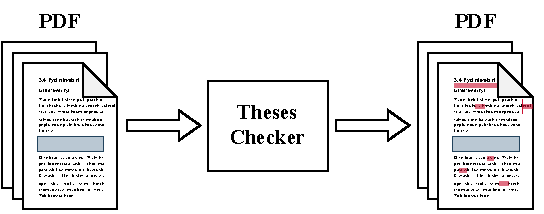
\includegraphics[width=\linewidth]{obrazky-figures/Theses_Checker_diagram.pdf}
    \caption{\todo{TODO: popis}}
\end{figure}

Vytvořená webová aplikace by měla odrážet tento uvedený vzor vstupů a~výstupů.
Úvodní stránka, jejíž náčrt lze vidět na
obrázku~\ref{pic_theses_checker_design_page1}, slouží pouze pro nahrání
PDF dokumentu, aby se mohl dále zpracovat. Po stisku tlačítka CHECK bude
PDF dokument zpracován, zkontrolován a~anotován. Poté bude uživatel přesměrován na
stránku jejíž náčrt je ukázán na obrázku~\ref{pic_theses_checker_design_page2}.
Na této stránce bude pro lepší uživatelskou přívětivost přímo zobrazen
anotovaný dokument místo často používaného odkazu na stáhnutí souboru.

\begin{figure}[H]
    \label{pic_theses_checker_design_page1}
    \centering
    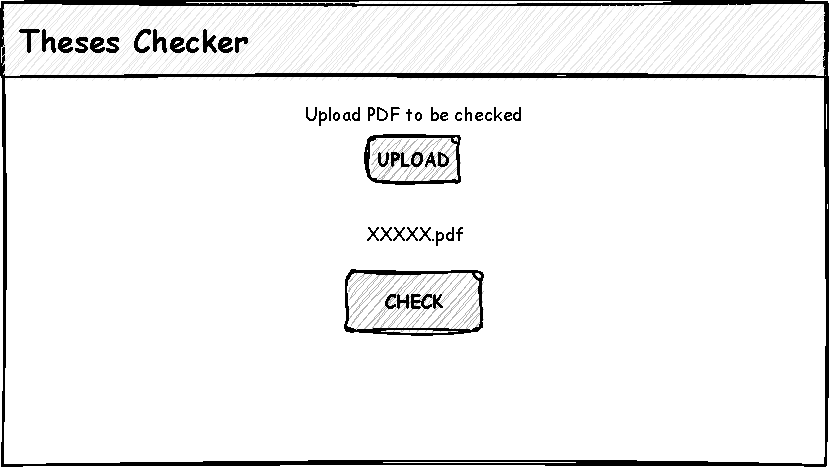
\includegraphics[width=0.8\linewidth]{obrazky-figures/Theses_Checker_design-page1.pdf}
    \caption{\todo{TODO: odkaz}}
\end{figure}

\begin{figure}[H]
    \label{pic_theses_checker_design_page2}
    \centering
    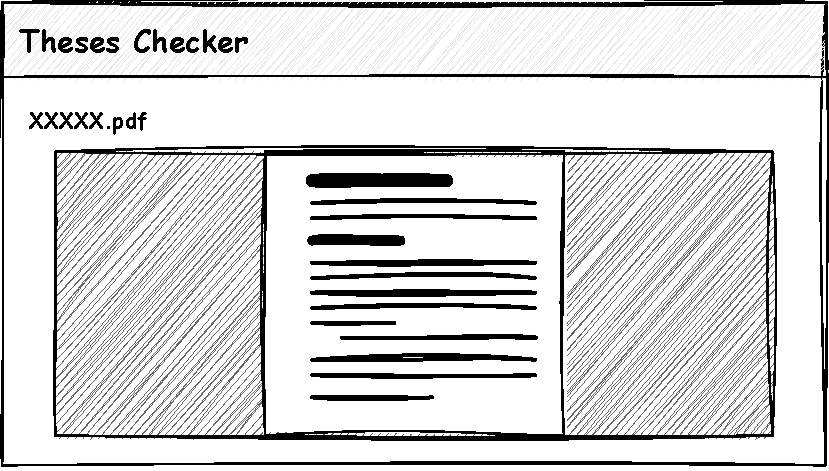
\includegraphics[width=0.8\linewidth]{obrazky-figures/Theses_Checker_design-page2.pdf}
    \caption{\todo{TODO: odkaz}}
\end{figure}

Výstupní dokument bude obsahovat několik anotací, pro označení nalezených chyb.
Toto označení by mělo být viditelné a~mělo by jasně označovat, co za chybu bylo
nalezeno. Z~tohoto důvodu bylo navrženo používání highlight anotace kombinovanou
s~pop-up anotací. Highlight anotace označí, kde na stránce byla nalezena chyba
a~podrobný popis nalezené chyby je možné zobrazit rozkliknutím pop-up anotace,
která se váže na danou highlight anotaci.

\todo{cílová skupina?, obrázek pop-up anotace?}

%#######################    4.3 Využité technologie    #######################
\section{Využité technologie}
Pro zpracování všech programových částí této bakalářské práce, byly
využity následující technologie:

\begin{description}
    \item[Python:] Jazyk Python byl zvolen, kvůli knihovně PyMuPDF
    (popsána v~sekci~\ref{python_libraries}), která splňuje nejvíce požadavků
    pro tuto práci. Některé z~požadavků jsou například úprava existujícího PDF
    souboru, přidání základních anotací, extrakce textu a~možnost exportovat
    libovolnou stránku PDF souboru na obrázek (v~tomto případě pixelovou mapu).
    Další funkcí, která byla velmi nápomocná je zjištění pozice některých
    objektů, které se vyskytují na stránce.

    \item[PythonAnywhere:] PythonAnywhere je služba poskytující hosting webových
    aplikací vytvořených v~jazyce Python. Je to jedna z~mála služeb poskytujících
    verzi 3.10 jazyka Python i~pro své neplatící uživatele. PythonAnywhere
    nabízí pět typů účtu a~mezi nimi je i~účet, který je zcela zdarma. Tento
    účet má několik omezení (např. omezení velikosti datového úložiště na
    512\,MB, bez možnosti používání vlastní domény a~nutnost alespoň jednoho
    přihlášení a~potvrzení činnosti v~intervalu 3~měsíců), ale pro
    implementovanou aplikaci je dostačující.

    \item[Django:] Django je jeden z~nejznámějších frameworků pro tvorbu webových
    aplikací v~jazyce Python. Tato volba byla závislá právě na vybraném
    programovacím jazyce a~též na službě PythonAnywhere, která má několik
    návodů na nasazení webových aplikací využívajících právě framework Django.
    Django dokumentace je velmi rozsáhlá a~obsahuje i~návod pro vytvoření
    první takové webové aplikace.
    
    \item[HTML, CSS:] HTML a~CSS jazyky byly použity pro grafickou tvorbu
    zobrazených webových stránek. Upravený jazyk HTML se používá pro tvorbu
    šablon využívaných v~Django frameworku. A~CSS jazyk byl použit pro
    definici grafického stylu zobrazených stránek.
    
    \item[JavaScript:] Jazyk JavaScript byl ve vyvinuté aplikaci použit pro
    částečnou kontrolu, zda je nahraný soubor formátu PDF. Další využití
    bylo pro zobrazení načítacího elementu (\uv{poskakujících} teček),
    které je viditelné při čekání na zpracování nahraného PDF dokumentu.
    
\end{description}



%#######################    4.4 Implementace webové aplikace    #######################
\section{Implementace webové aplikace}
Výsledná webová aplikace byla vyvinuta s~pomocí Django frameworku.
Nahraný soubor se pošle na server pomocí HTTP požadavku metodou POST
a~uloží se ve specifické složce. Poté se pomocí třídy \texttt{Checker}
uložené v~souboru \texttt{theses\_checker.py} (popsáno dále
v~kapitole~\ref{checker}) zkontroluje a~přidají se anotace.
Tento výstupní soubor se opět uloží na server do určité složky a~původní soubor
se ze serveru odstraní. Následně bude uživatel přesměrován na stránku, která
zobrazí výstupní anotovaný dokument. Po zobrazení tohoto dokumentu na stránce je
dokument odstraněn ze serveru. Postup zpracování nahraného PDF souboru je
naznačen na obrázku~\ref{pic_communication}.

\begin{figure}[H]
    \label{pic_communication}
    \centering
    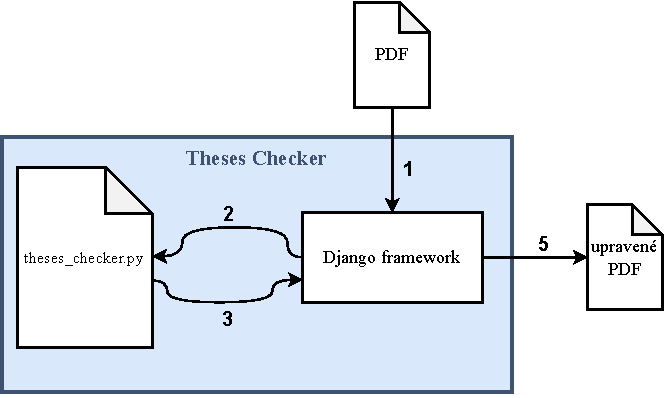
\includegraphics[width=0.8\linewidth]{obrazky-figures/Theses_Checker_communication.pdf}
    \caption{TODO: popis + odkaz}
\end{figure}

\begin{figure}[H]
    \label{pic_theses_checker_page1}
    \centering
    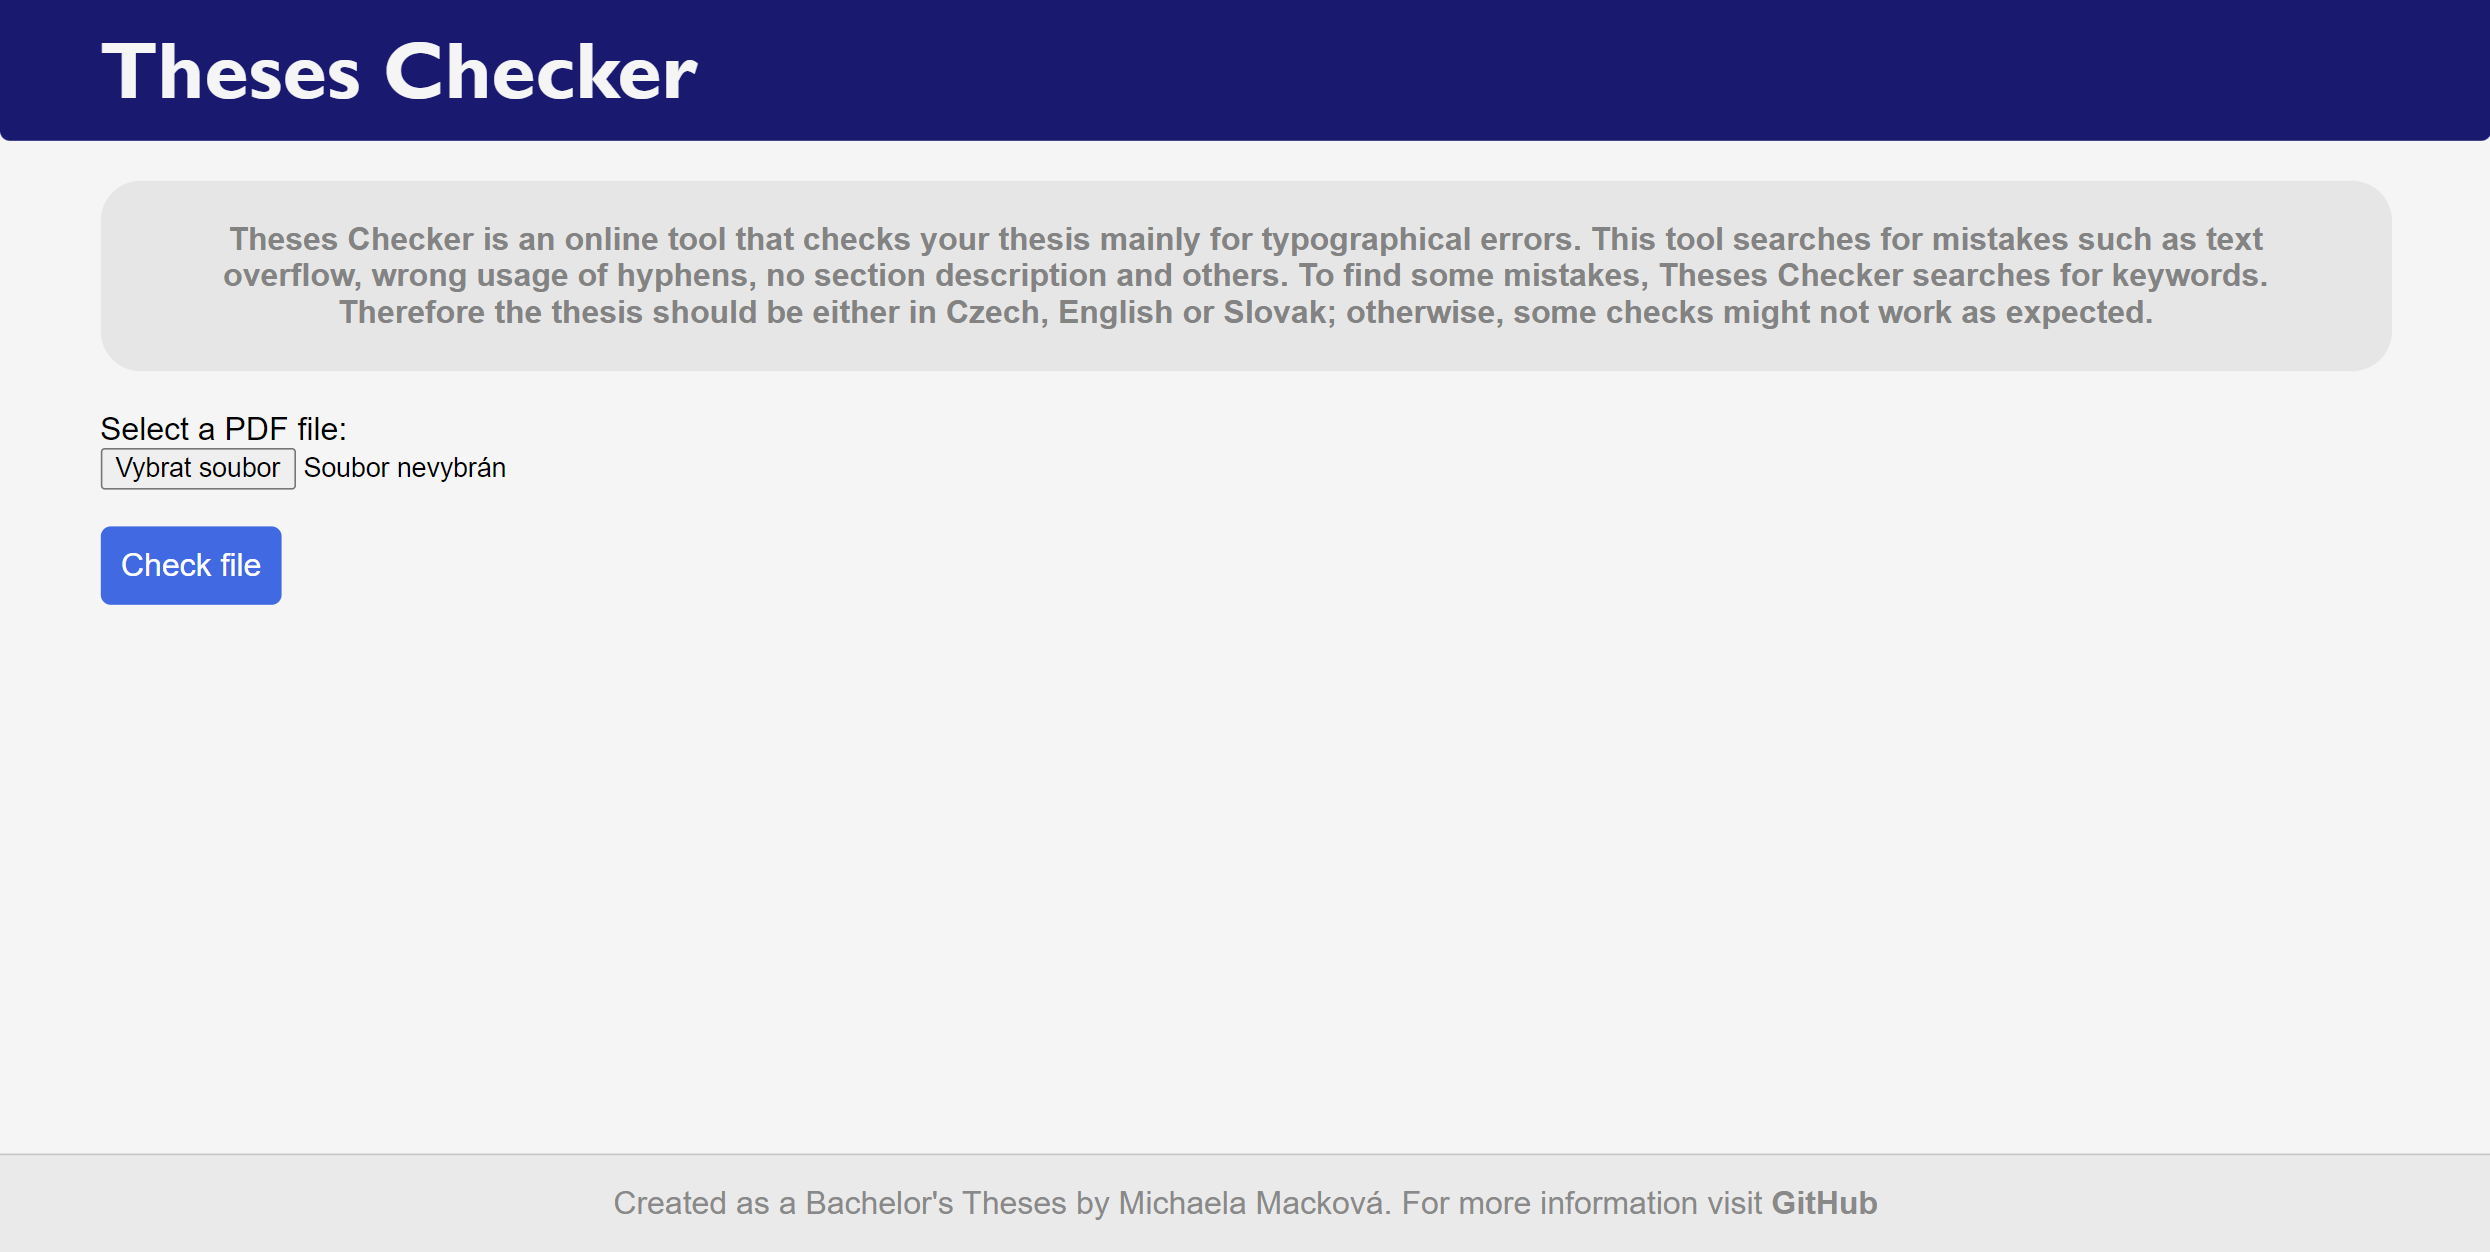
\includegraphics[width=\linewidth]{obrazky-figures/screenshot-page1.png}
    \caption{\todo{TODO: odkaz}}
\end{figure}

\begin{figure}[H]
    \label{pic_theses_checker_page1_loading}
    \centering
    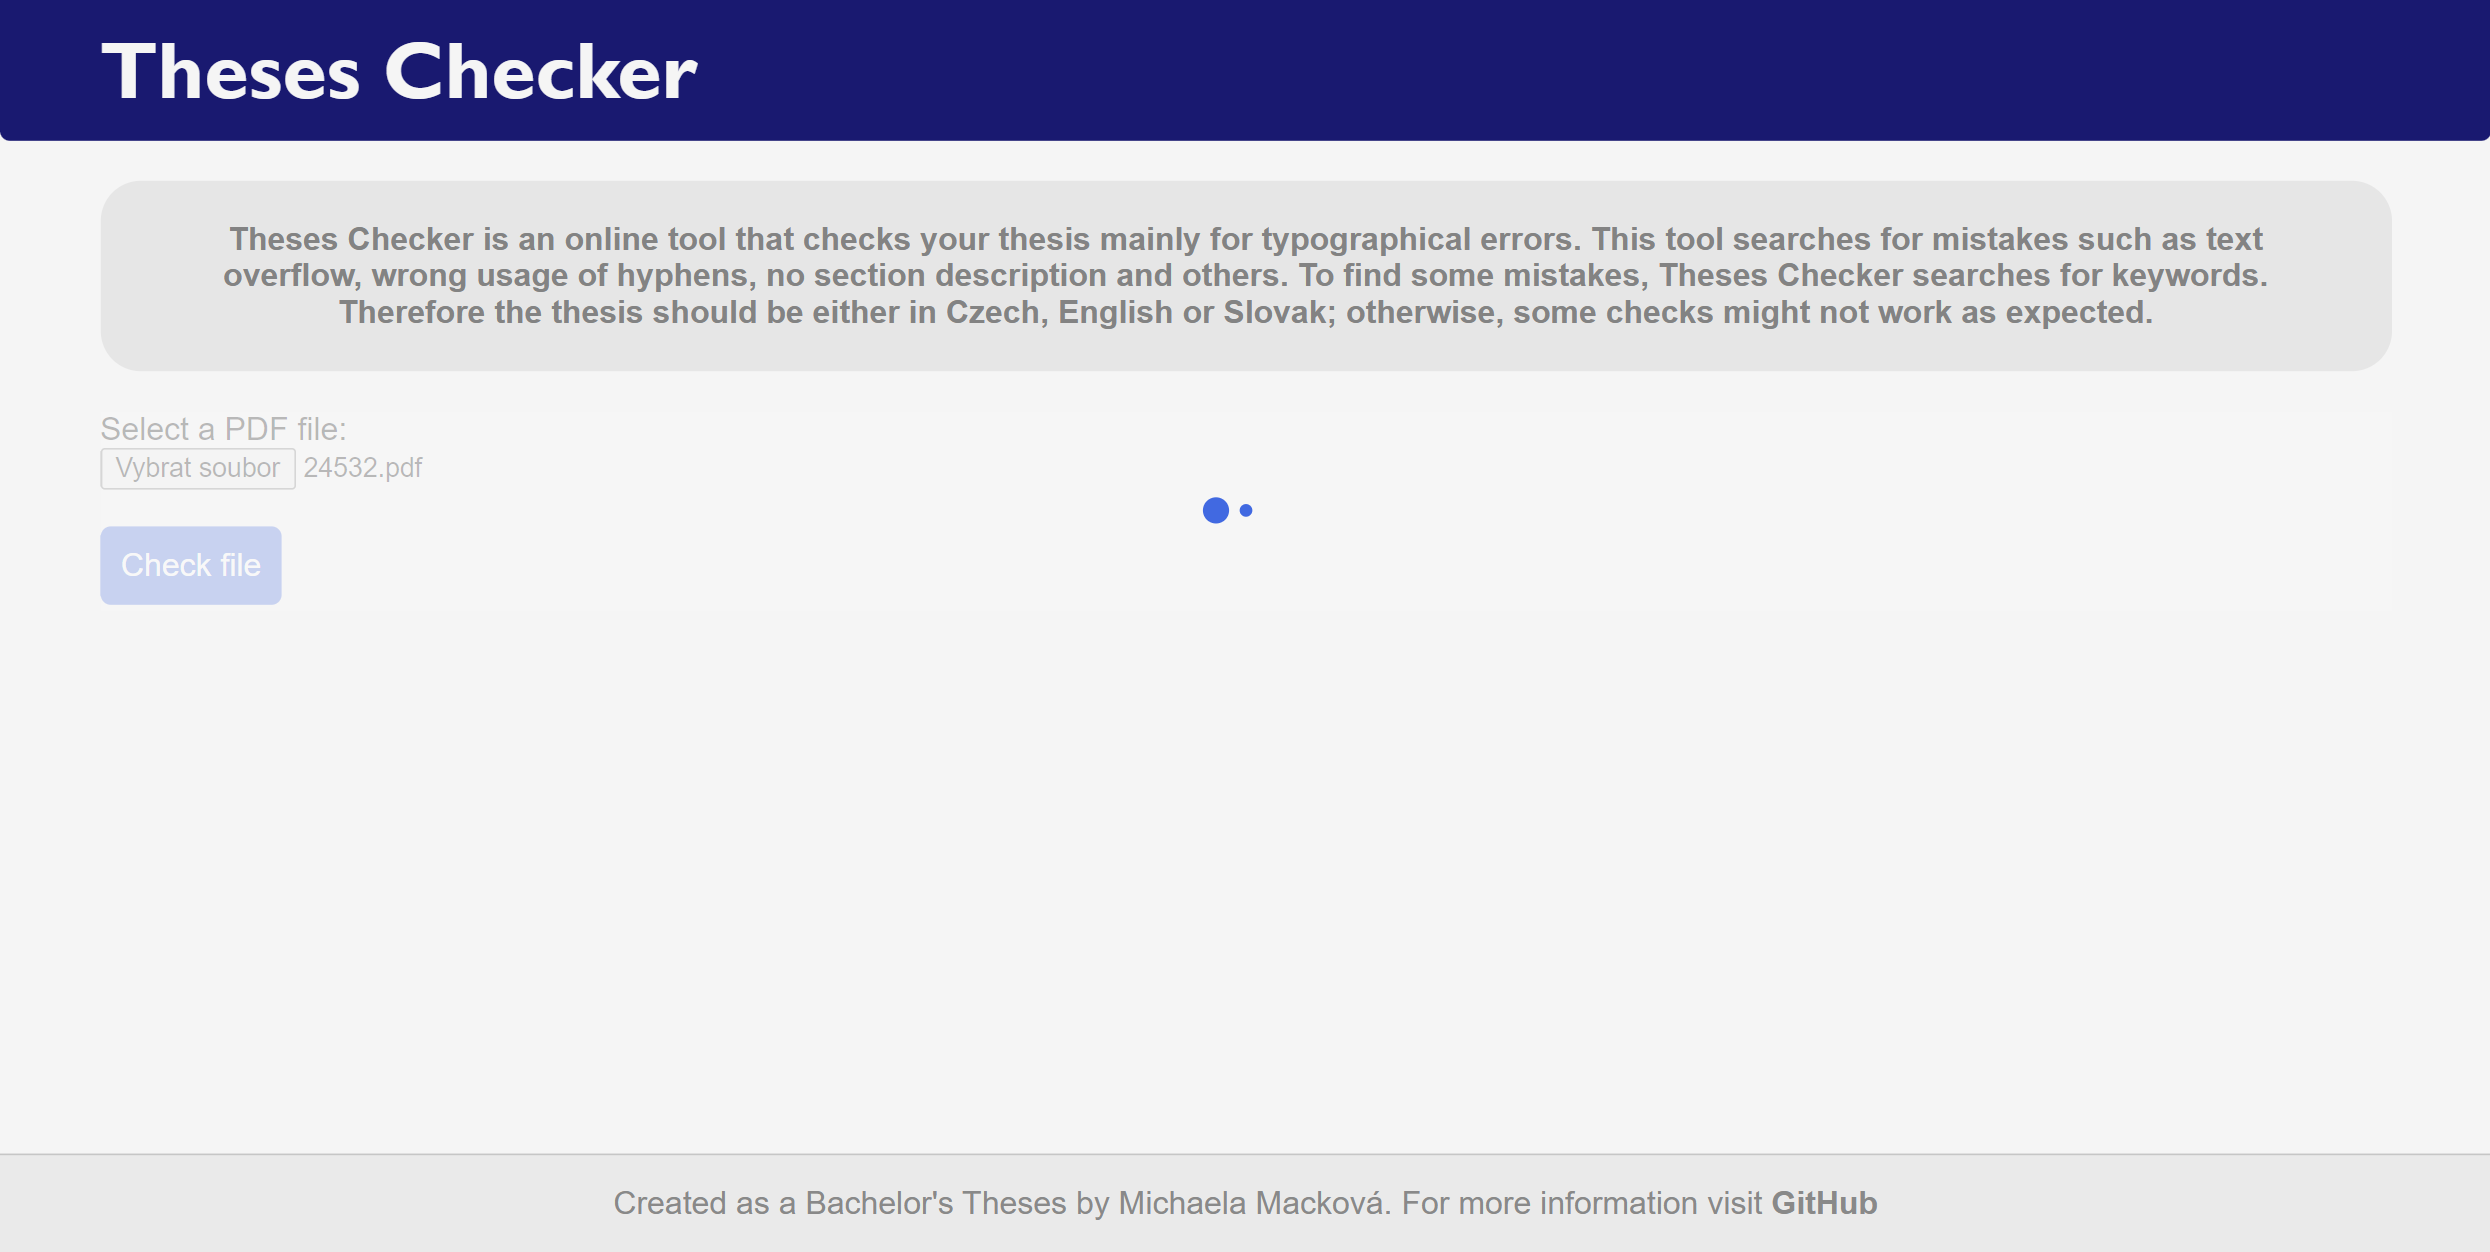
\includegraphics[width=\linewidth]{obrazky-figures/screenshot-loading.png}
    \caption{\todo{TODO: odkaz}}
\end{figure}

\begin{figure}[H]
    \label{pic_theses_checker_page2}
    \centering
    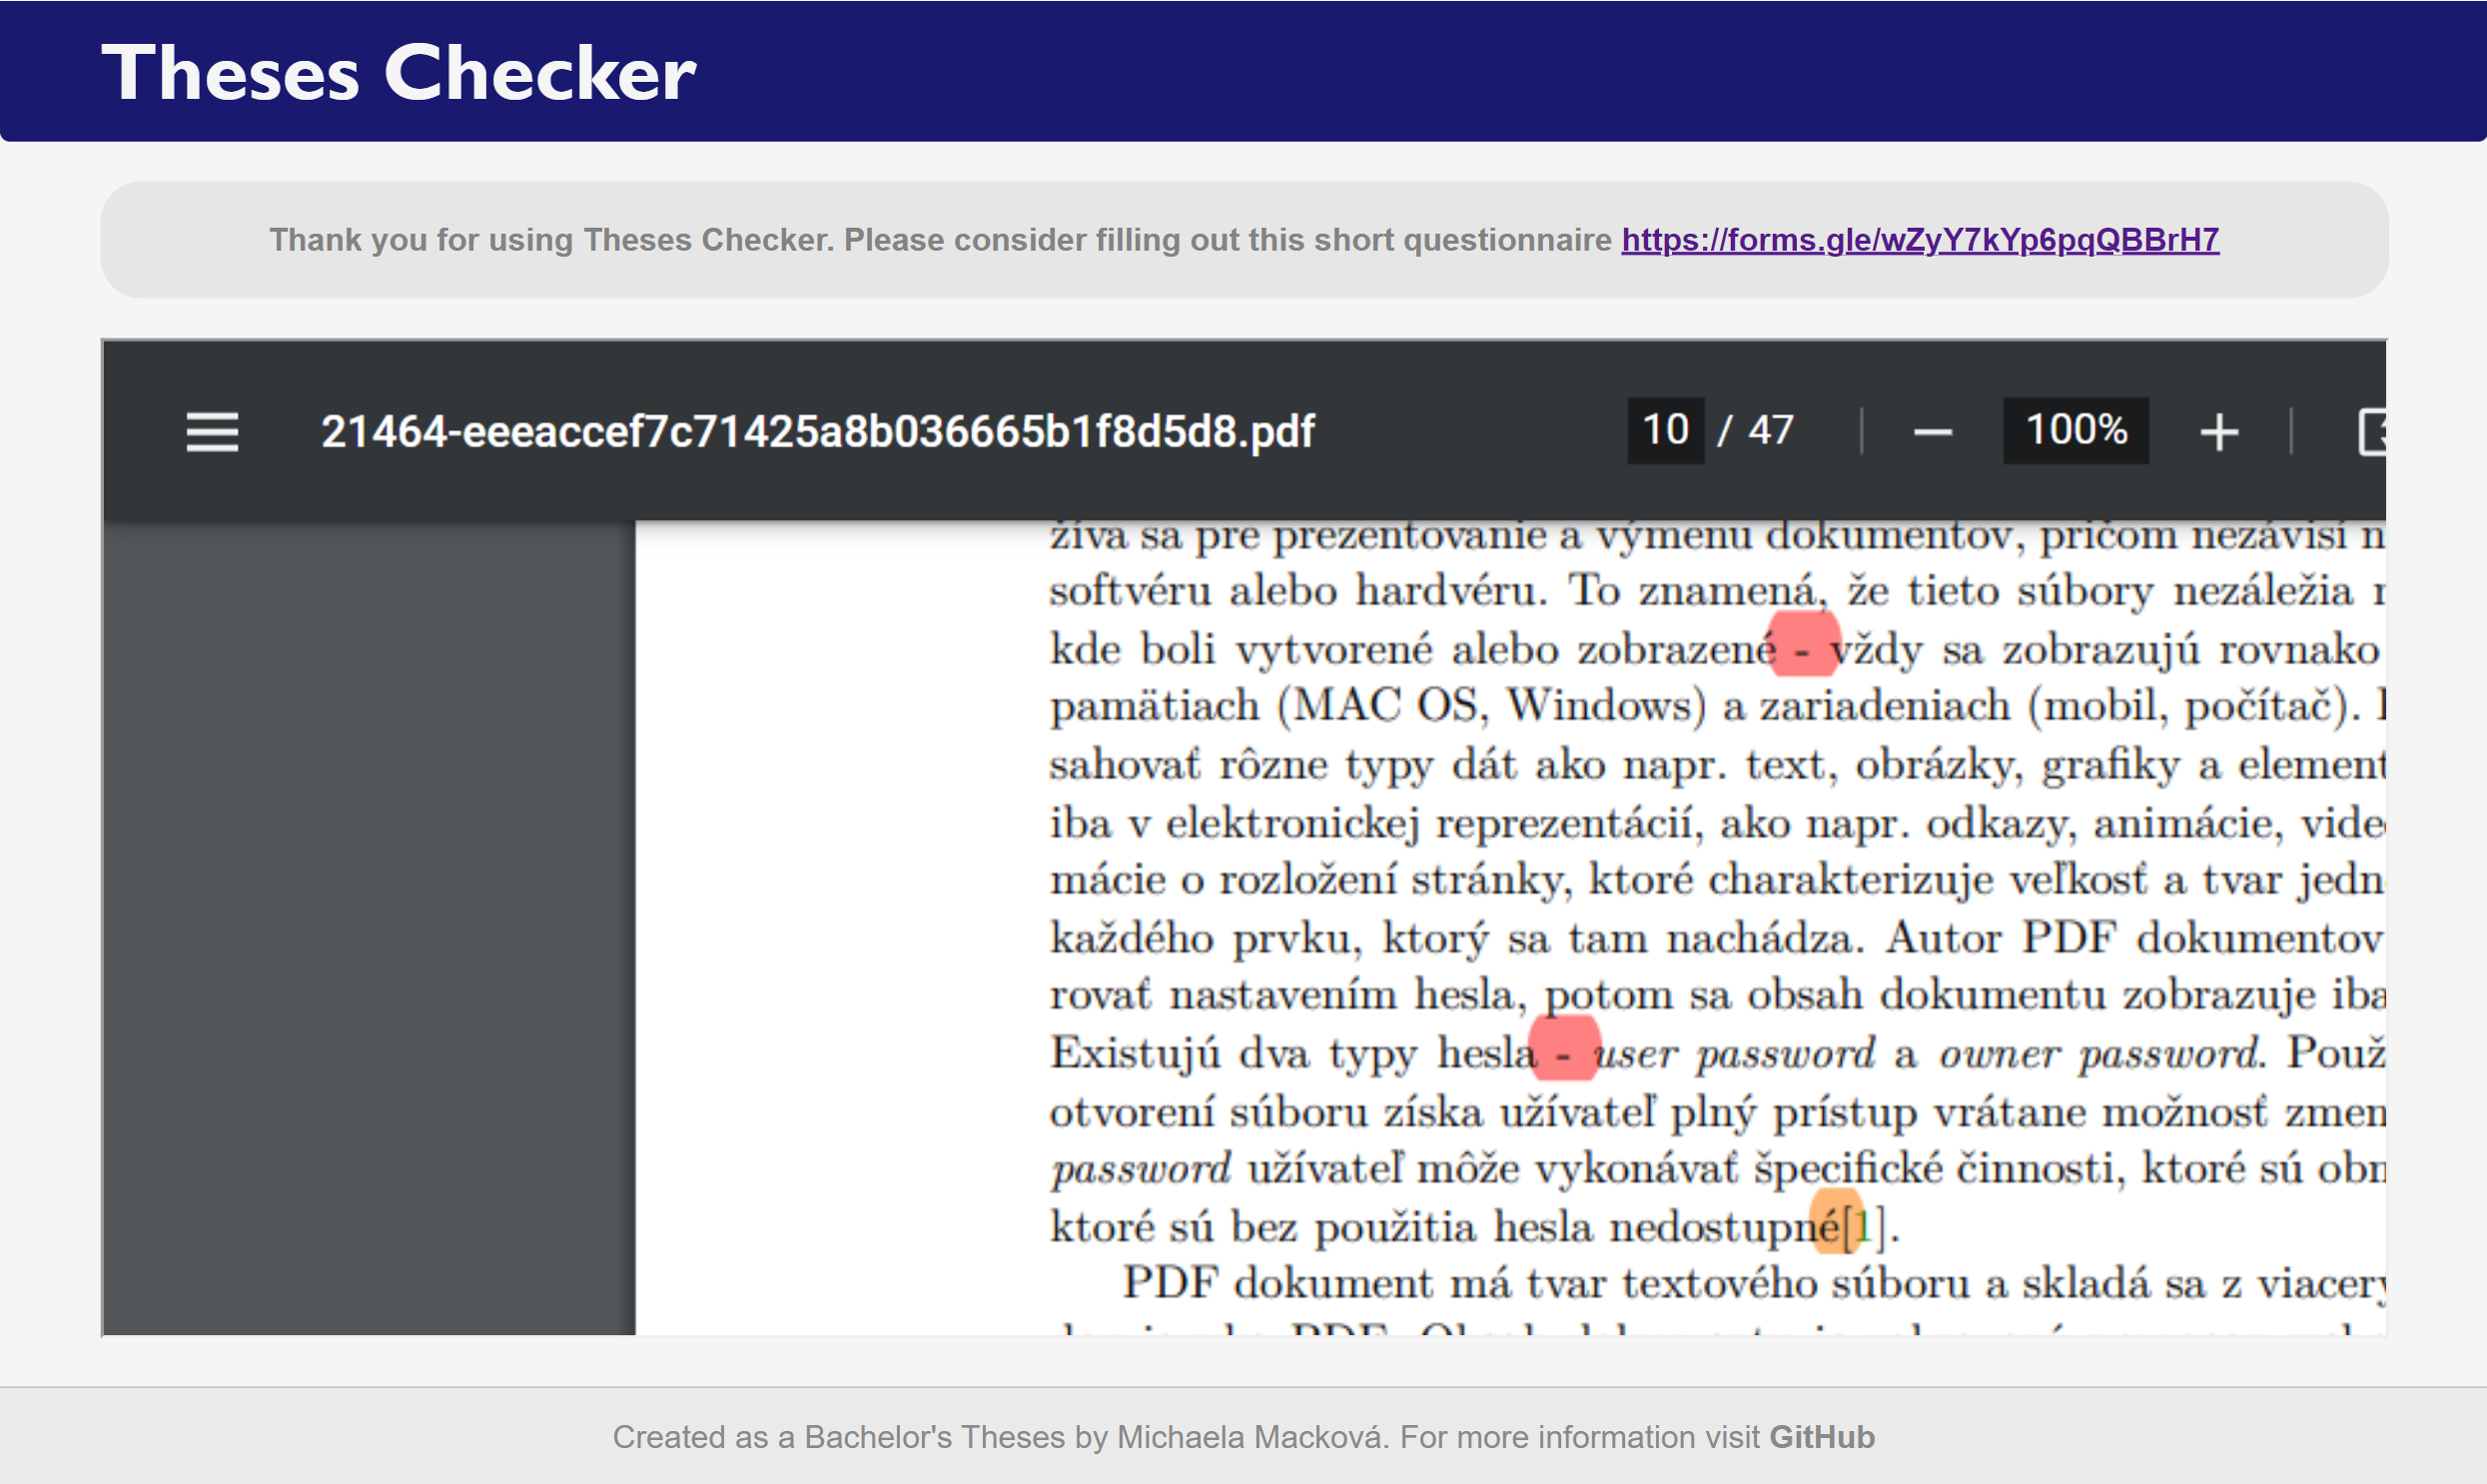
\includegraphics[width=\linewidth]{obrazky-figures/screenshot-page2.png}
    \caption{\todo{TODO: odkaz}}
\end{figure}


%---------- 4.4.1 Architektura webové aplikace ----------
\subsection*{Architektura webové aplikace}
\todo{MVC?, kde jsou jaké soubory, }


\dummyText[2]


%---------- 4.4.2 Implementační detaily ----------
\subsection*{Implementační detaily}
\todo{error views, vymazání anotovaného souboru, }

\dummyText



%#######################    4.5 Program pro vyhledání chyb a jejich následné vyznačení    #######################
\section{Program pro vyhledání chyb a~jejich následné vyznačení} \label{checker}
Program, který zodpovídá za práci s~PDF dokumentem, je obsažen v~souboru s~názvem
\texttt{theses\_checker.py}. Pro zkontrolování technické zprávy se musí použít
funkce \texttt{annotate()} ze třídy \texttt{Checker}. Při vytváření instance této
třídy se musí uvést cesta ke kontrolovanému PDF souboru. Třída \texttt{Checker}
v~sobě obsahuje všechny potřebné funkce a~proměnné pro správnou funkci hledání
a~zvýrazňování chyb uvnitř PDF dokumentů.

Třídní proměnné jsou rozděleny do dvou skupin -- statické třídní proměnné
a~třídní proměnné vázané na jednu instanci. Statické třídní proměnné nemění 
svou přiřazenou hodnotu a~jsou využívány především pro jednotnou barvu označení
nalezených chyb. Jsou to proměnné:
\begin{itemize}
    \item \texttt{RND\_PAGE\_CNT} -- Tato proměnná se používá při zjišťování
    základních informací o~dodaném PDF dokumentu. Tyto informace jsou potřebné
    pro správné hledání chyb. Proměnná obsahuje maximální počet náhodných stran,
    které jsou zkoumány, pro získání těchto základních informací.

    \item \texttt{HIGH\_RED} -- Proměnná obsahuje červenou barvu pro zvýraznění
    textu při nalezené chybě. Barva je ve formátu RGB\footnote{
        Formát RGB -- Uspořádaná trojice, kde každý prvek obsahuje celé číslo
        v~intervalu $<0;255>$.
    }.

    \item \texttt{HIGH\_ORANGE} -- Je to oranžová barva ve formátu RGB pro
    zvýraznění textu při varování.
    
    \item \texttt{HIGHLIGHT\_PADDING} -- Tato proměnná obsahuje velikost okraje,
    který je použit, když je zvýraznění moc těsné zvýrazněnému objektu. Toto
    nastává při hledání přetečení okraje stránky.
    
    \item \texttt{RED} -- Je to červená barva ve formátu RGB. Tato barva je
    použita při kreslení přímek.
    
    \item \texttt{WHITE} -- Proměnná obsahuje bílou barvu ve formátu RGB.
\end{itemize}
Třídní proměnné instance během programu mění svou hodnotu. Některé jsou využívány
pro navigaci v~kontrolovaném dokumentu a~další v~sobě mají uložená data
o~tomto dokumentu, která jsou potřebná k~prováděným kontrolám. Některé z~důležitých
proměnných jsou:
\begin{itemize}
    \item \texttt{mistakes\_found} -- Veřejná proměnná typu boolean, která označuje,
    zda byla při kontrole PDF dokumentu nalezena jakákoliv chyba (či varování
    na chybu).

    \item \texttt{borderNotFound} -- Tato proměnná je veřejná a~označuje zda byl
    při hledání základních informací o~dokumentu nalezen okraj stránky. 

    \item \texttt{\_\_document} -- Tato privátní proměnná obsahuje instanci
    kontrolovaného PDF dokumentu.

    \item \texttt{\_\_currPage} -- Privátní proměnná, která obsahuje instanci
    aktuálně zpracovávané stránky z~PDF dokumentu.
    
    \item \texttt{\_\_currTextPage} -- Tato privátní proměnná obsahuje instanci
    takzvané \emph{textpage} aktuálně zpracovávané stránky. Textpage se používá
    pro urychlení některých funkcí pracující s~PDF stránkou.
    
    \item \texttt{\_\_currPixmap} -- Tato privátní proměnná obsahuje pixelovou
    mapu aktuálně skenované stránky. Pixelová mapa je podobná obrázku a~v~tomto
    programu se používá pouze pro nalezení přetékajících objektů za okraje
    aktuálně kontrolované stránky.
    
    \item \texttt{\_\_currDict} -- Tato privátní proměnná obsahuje aktuálně
    zkoumanou stránku ve formě slovníku, jehož struktura je uvedena na
    obrázku~\ref{pic_curr_page_dict}.
    \begin{figure}[H]
        \label{pic_curr_page_dict}
        \centering
        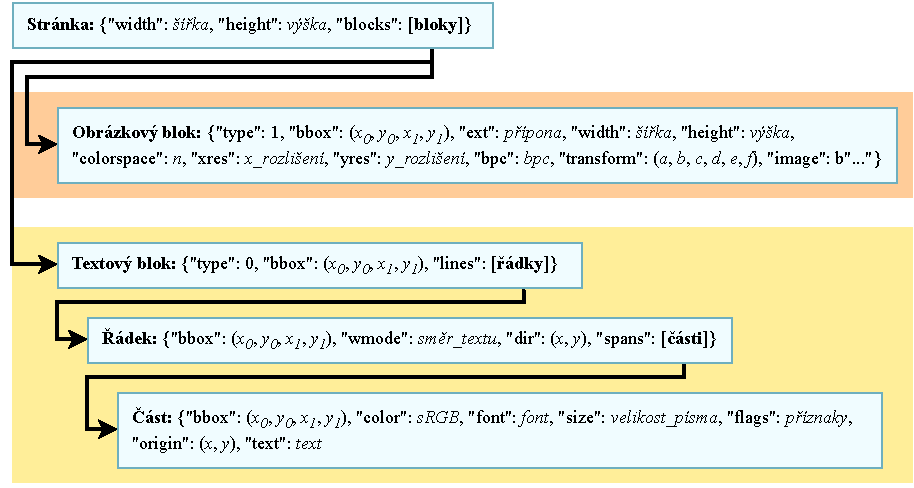
\includegraphics[width=\linewidth]{obrazky-figures/page_dictionary.pdf}
        \caption{TODO: \url{https://pymupdf.readthedocs.io/en/latest/textpage.html}}
    \end{figure}
    
    \item \texttt{\_\_currPageEmbeddedPdfs} -- Privátní proměnná, která obsahuje
    seznam vykreslených vložených PDF na aktuálně zpracovávané stránce. Každá
    položka tohoto seznamu je pro kompatibilitu s~proměnnou \texttt{\_\_currDict}
    typu slovník, který odpovídá slovníku \emph{Image block} uvedeném na
    obrázku~\ref{pic_curr_page_dict}. 
    
    \item \texttt{\_\_currPageTextContent} -- Tato privátní proměnná obsahuje
    všechen text vyskytující se na aktuální stránce. Jelikož při extrakci textu
    z~PDF stránky nelze vždy získat nepřerušovaný text (text většinou obsahuje
    například znak
    zalomení řádku tam, kde by byl vykreslen na stránce), musí se nejdříve tento
    extrahovaný text upravit.
    Text obsažen uvnitř proměnné \texttt{\_\_currPageTextContent} je formátován
    přímo pro čtení (falešné nové řádky nahrazeny za mezeru a~jsou odebrány
    spojovníky u~rozdělených slov např. \emph{spojo-vník}), kde každý blok je
    oddělen prázdným
    řádkem.\todo{TODO: samotná podsekce?, proměnná obsahuje i text z vložených pdf}
\end{itemize}

Než se budou moct provézt některé kontroly, musí se nejdříve zjistit pár
základních informací o~kontrolovaném dokumentu (například font normálního textu
nebo souřadnice okrajů stránek). Toto získávání informací provádí funkce
\texttt{\_\_getDocInfo()}, která pro zrychlení programu skenuje pouze předem
určený počet stran. Skenované stránky jsou získány náhodně.

% \lstinputlisting[
%     style=myPython,
%     caption={TODO:},
%     label=code
% ]{code_examples/python_code/getDocInfo.py}

Hlavní funkce \texttt{annotate()} (naznačená ve výpisu~\ref{code_annotate}) přijímá parametry typu boolean, kde
každý typ kontroly má vlastní parametr. Tyto parametry určují, zda se má daná
kontrola provést, či nikoliv. Další parametry, které tato funkce přijímá jsou
\texttt{annotatedPath}, který určuje cestu pro vytvořený anotovaný soubor,
a~\texttt{embeddedPdfAsImage}, který je typu boolean a~označuje, zda se mají
při kontrolách chovat vložené PDF soubory jako obrázky, nebo jako pokračování
daného PDF dokumentu. Tato funkce provádí všechny kontroly a~vše s~nimi spojené.
To znamená zjištění potřebných informací, samotná kontrola a~označení nalezených
chyb. Každá kontrola má vlastní funkci, která prozkoumá jednu stránku a~nalezené
chyby označí pomocí PDF anotací (vysvětleny v~sekci~\ref{PDF_annotations}).
Chyby které program umí zkontrolovat jsou přetečení za okraj stránky, 
špatné použití spojovníku, nevhodná šířka obrázku, vynechaná mezera před levou
závorkou, chybějící text mezi názvy sekcí a~odkaz na neexistující referenci.

\noindent\begin{minipage}{\linewidth}
    \hfill
    \lstinputlisting[style=myPython,caption={TODO:},label=code_annotate]{code_examples/python_code/annotate.py}
\end{minipage}



%---------- 4.6.1 Extrahovaný text ve formátu pro čtení ----------
\subsection*{Extrahovaný text ve formátu pro čtení}
\todo{proč existuje proměnná \texttt{\_\_currPageTextContent} a na co se to potom používá}


%---------- 4.6.1 Nalezení okraje stránky ----------
\subsection*{Nalezení okraje stránky}
Hlavní kontrola, na kterou se měl tento program zaměřit je přetékání objektů za
okraj stránky. Pokud jsou známy souřadnice okraje, nalezení jeho přetečení
se řídí algoritmem naznačeném ve výpisu~\ref{code_overflow}.

\noindent\begin{minipage}{\linewidth}
    \hfill
    \lstinputlisting[
        style=myPython, caption={TODO:}, label=code_overflow
    ]{code_examples/python_code/overflow.py}
\end{minipage}

PDF dokument nemusí mít uloženou informaci o~souřadnicích okraje stránky. Pro
jeho nalezení se tak musí daná informace nalézt z~již vykreslené stránky.
Použitá knihovna PyMuPDF obsahuje funkce, díky kterým lze zjistit polohu
vykreslených objektů a~podobjektů (například obrázků, bloků textu a~řádků v~nich
obsažených). Pokud blok textu obsahuje přetečení, ohraničení celého bloku
obsahuje i~toto přetečení (viz obrázek~\ref{pic_block_bbox}).

\begin{figure}[H]
    \label{pic_block_bbox}
    \centering
    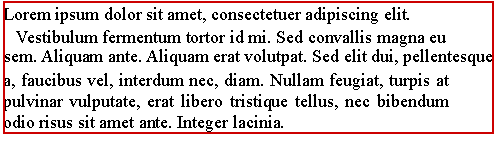
\includegraphics[width=0.7\linewidth]{obrazky-figures/block_bbox.pdf}
    \caption{Obrázek ukazuje červeně označené ohraničení bloku textu, který obsahuje přetečení.}
\end{figure}

Při hledání okraje stránky je použitý algoritmus inspirován tím, jak takový
okraj hledá člověk. Prozkoumá se každý řádek textu, který se vyskytuje na
stránce a~uloží se souřadnice jeho levého i~pravého okraje. Za okraj stránky se
poté považuje medián těchto uložených okrajů řádků. První řádek v~odstavci 
může být odsazený, a~proto se pro větší přesnost tohoto algoritmu (uvedeného
ve výpisu~\ref{code_get_page_border}) neukládá do potenciálních levých okrajů.
Podobné pravidlo platí i~pro poslední řádek a~jeho pravý okraj.

\noindent\begin{minipage}{\linewidth}
    \hfill
    \lstinputlisting[style=myPython, caption={TODO:}, label=code_get_page_border]{code_examples/python_code/getPageBorder.py}
\end{minipage}

\todo{?blbne u textových objektů (tabulka, listing, grafy?)?}

 

%---------- 4.6.2 Nalezení souřadnic vloženého PDF na stránce ----------
\subsection*{Nalezení souřadnic vloženého PDF na stránce}
V~technické zprávě se často vyskytují obrázky. Jak je řečeno 
v~podkapitole~\ref{vector_graphic}, je vhodné používat vektorovou grafiku
pro grafy a~schémata. Vektorové obrázky mohou mít formát PDF a~ty se poté
vkládají do PDF dokumentu technické zprávy. Při zpracovávání tohoto PDF dokumentu
se nijak nerozlišuje mezi interními částmi původního PDF dokumentu a~vloženého
PDF obrázku. Kontroly určené pro obrázky tedy nezahrnují tyto vložené PDF
a~kontroluje se pouze text uvnitř těchto obrázků.

Aby se s~vloženým PDF mohlo pracovat jako s~obrázkem, musí se zjistit
jeho poloha na stránce. Ve formátu PDF nejsou nikde přímo uvedeny souřadnice
vloženého PDF obrázku. Obrázek ve formátu PDF je uvnitř PDF dokumentu uložen
jako XObject (popsaný v~podkapitole~\ref{XObject}) a~jak je na dané stránce
vykreslen je popsáno v~toku content stream (více lze nalézt
v~sekci~\ref{content_streams}) té stejné stránky.
Pro zjištění souřadnic vykresleného obrázku tedy program simuluje
stavy datové struktury graphics state, jenž je popsána
v~podkapitole~\ref{graphics_state}. Přesněji stačí simulovat parametr
CTM (current transformation matrix), ve kterém je uvedena matice pro transformaci
z~uživatelského prostoru do prostoru zařízení. Podtyp objektu XObject, který se
nejčastěji používá pro PDF obrázky, je typ Form XObject.

Příkazy uvedené
v~content streamu, které ovlivňují, jak bude objekt typu Form XObject vykreslen,
jsou \texttt{q} a~\texttt{Q} (manipulace s~graphics state zásobníkem),
\texttt{cm} (změna parametru CTM) a~\texttt{Do} (příkaz pro vykreslení
objektu XObject). Příkazem \texttt{cm} jsou prováděny elementární transformace
obrázku pro jeho správné napolohování na stránce. Jelikož matice CTM musí vždy
vyjadřovat transformaci z~jednoho prostoru do druhého a~příkazy \texttt{cm}
s~touto maticí manipulují, podle dříve uvedeného
vzorce~\eqref{multiple_matrix_transformations} si dokážeme odvodit
vzorec~\eqref{cm_multiplication}. V~tomto vzorci vyjadřuje matice $CTM$
aktuální hodnotu CTM uložené uvnitř graphics state, $M_{cm}$ 
je matice, kterou vyjadřuje operand použitého příkazu \texttt{cm}
a~matice $CTM'$ je výsledná matice, jejíž hodnota je nově uložena do
CTM parametru datové struktury graphics state.
\begin{equation} \label{cm_multiplication}
    CTM' = M_{cm} \cdot CTM
\end{equation}

Pro získání takových souřadnic obrázku, aby se s~nimi mohlo dále pracovat
ve vytvořeném programu, se získané souřadnice musí ještě transformovat
maticí stránky. Tato matice lze získat přímo jako atribut
\texttt{transformation\_matrix} proměnné \texttt{\_\_currPage}.
Stejného výsledku lze dosáhnout, když před získáním souřadnic obrázku pomocí
vynásobení matice CTM, získáme přímo matici transformace obrázku do našeho
vyžadovaného prostoru. Toto je vyjádřeno
v~rovnici~\eqref{picture_transformation_matrix}, kde $CTM$ je aktuální hodnota
parametru CTM ze struktury graphics state, $M_T$ je matice stránky a~$M_{PT}$
je kombinovaná matice transformace obrázku.
\begin{equation} \label{picture_transformation_matrix}
    M_{PT} = CTM \cdot M_{T}
\end{equation}

Použitý algoritmus pro získání souřadnic všech vnořených PDF objektů,
vykreslených na aktuální stránce je naznačen ve vývojovém diagramu na
obrázku~\ref{pic_embedded_pdf_flow_chart}.

\begin{figure}[H]
    \label{pic_embedded_pdf_flow_chart}
    \centering
    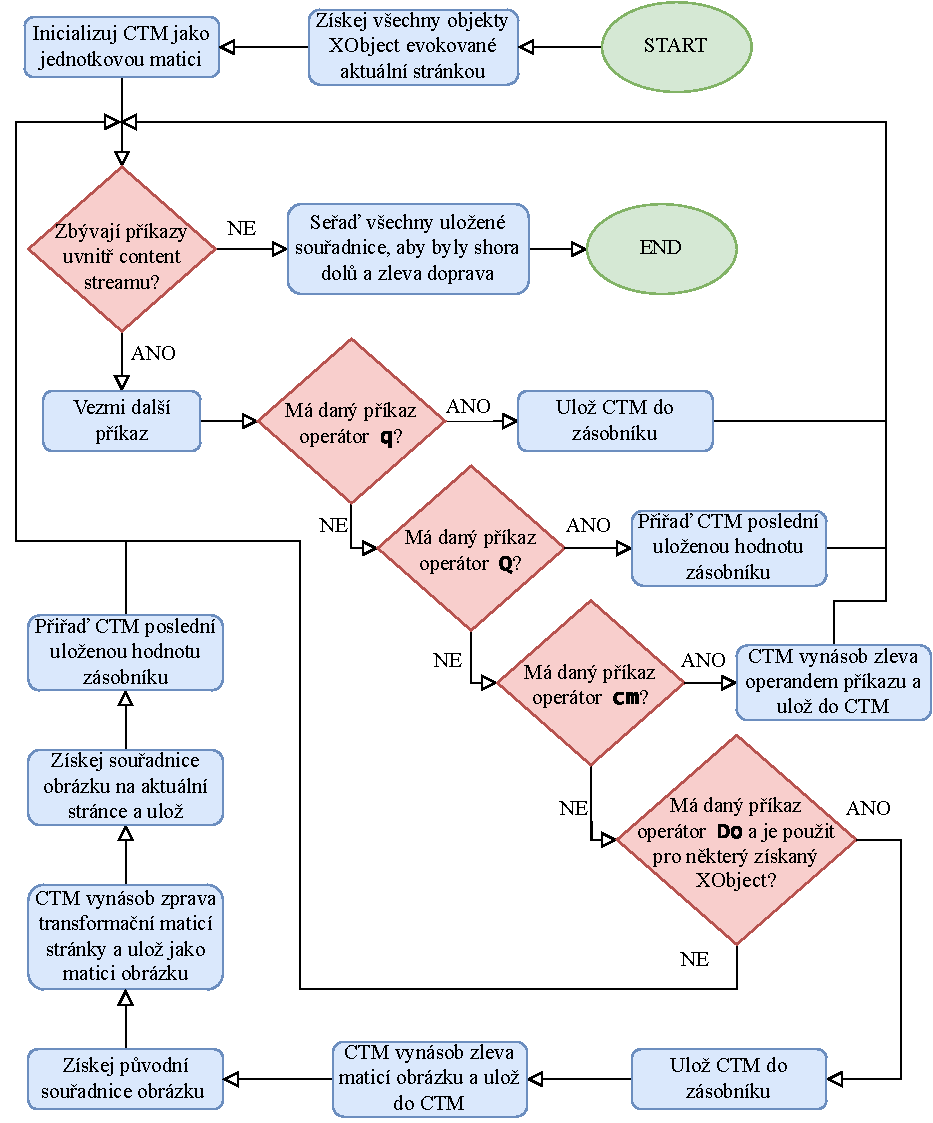
\includegraphics[width=\linewidth]{obrazky-figures/embedded_pdf_flow_chart.pdf}
    \caption{TODO: popis + odkaz}
\end{figure}



%#######################    4.7 Ukázka použití vytvořené webové aplikace    #######################
\section{Ukázka použití vytvořené webové aplikace}

\dummyShortText[13]

\dummyText

\todoimage{width=\linewidth,height=3.3in}{Zvolení PDF a~filtrů na webu.}

\dummyShortText[8]

\todoimage{width=\linewidth,height=3.3in}{Čekání na webu.}

\dummyText

\todoimage{width=\linewidth,height=3.3in}{Anotované PDF na webu.}


%#######################    4.7 Doplňující program pro použití v~příkazovém řádku    #######################
\section{Doplňující program pro použití v~příkazovém řádku}

Implementovaná webová aplikace umí najednou kontrolovat pouze jeden nahraný PDF
soubor. Vedoucí diplomových prací často potřebují zkontrolovat více takových
souborů, proto byl navíc vytvořen program použitelný v~příkazovém řádku. 
Tento program je v~souboru \texttt{check.py} a~používá program ze
sekce~\ref{checker}. Pro správnou funkčnost musí být tyto dva soubory uloženy ve
stejné složce. Program umí na jeden příkaz kontrolovat více PDF souborů
a~s~pomocí nepovinných přepínačů \texttt{-o}, \texttt{-i}, \texttt{-H}, 
\texttt{-t}, \texttt{-s}, \texttt{-e} a~\texttt{-b} lze určit které kontroly
budou či nebudou probíhat. Tento script podporuje navíc nepovinný přepínač
\texttt{--embedded\_PDF}, který určuje zda budou vnořené PDF brány jako
vektorové obrázky.

\todo{ukázka použití}

\subsection*{Závislosti}
Aby mohla být aplikace použitelná potřebuje následující:
\begin{itemize}
    \item Python\,==\,3.10.7
    \item PyMuPDF\,==\,1.20.2
    \item numpy\,==\,1.23.5
\end{itemize}
Jiné verze těchto závislostí nebyly testovány.


%*********************************************************************************




%*********************************************************************************
%                                 5 TESTOVÁNÍ 
%*********************************************************************************
%TODO: přejmenovat
\chapter{Testování a~zhodnocení výsledné aplikace}
\todo{TODO: úvod do kapitoly}

\dummyShortText[10]


%#######################    5.1 Ověření správné funkcionality vyhledávání chyb    #######################
\section{Ověření správné funkcionality vyhledávání chyb}
Již během prvních funkčních prototypů byla testována přesnost hledání
chyb. Toto testování probíhalo na zveřejněných diplomových prací, které byly
vytvořeny na Fakultě informačních technologií Vysokého učení technického v~Brně.
Tyto práce byly poskytnuty jako vstupy do programu a~jejich anotované
výstupy byly zkontrolovány ručně. Dále byly tyto výstupy kontrolovány
s~poskytnutými posudky oponenta.

Další vstupní data byla poskytnuta doktorem Tomášem Miletem. Tyto data
byly rozpracované práce z~minulých let, které měli doktora Mileta jako
vedoucího. Ke každé takové práci byla vždy poskytnuta její původní forma
a~její upravená forma obsahující poznámky ke zlepšení. Postup testování
na těchto rozpracovaných pracích bylo podobné jako na již zveřejněných, 
jen tyto výstupy z~vytvořené aplikace nebyly porovnávány s~posudkem oponenta,
ale s~poskytnutými poznámkami.


%#######################    5.2 Známé chyby aplikace    #######################
\section{Známé chyby aplikace}
Typografická kontrola zahrnuje velmi rozšířenou oblast a~často se váže k~jazyku
vypracovaného textu.
\todo{TODO: mezera před levou závorkou u funkcí a rovnic, okraje stránky pro oboustranný tisk, špatné ukazování chbějícího popisu kapitoly u grafů, tabulek atd., nefunguje na mobilních zařízeních}


%#######################    5.3 Uživatelské dotazníky    #######################
\section{Uživatelské dotazníky}
... 
Na dotazník odpovědělo celkem 26~uživatelů a~obsahoval tyto otázky:
\begin{itemize}
    \item Pomocí jakého prohlížeče jste aplikaci použili?
    \item Dokázali jste pomocí aplikace Theses Checker zkontrolovat svou
    diplomovou práci?
    \item Dokázali jste jednoduše nahrát PDF soubor?
    \item Zhodnoťte přehlednost označení chyb ve výsledném PDF
    \item Zobrazují se vám pop-up anotace?
    \item Bylo něco špatně označeno jako chyba?
    \item Jaký typ chyby byl špatně označen?
    \item Byla práce s webovou stránkou jednoduchá?
    \item Máte nějaké nápady na rozšíření či vylepšení?
\end{itemize}

Odpovědi na tento dotazník pomohly vylepšit funkcionalitu vytvořené aplikace.
Hlavní ... tohoto dotazníku bylo ověření již vytvořených kontrol a~určení,
jak je daná aplikace přehledná. Přehlednost označení nalezených chyb
uvnitř PDF dokumentu, mělo většinově dobré ohlasy, což lze
vyčíst z~obrázku~\ref{rate_checks}.

\begin{figure}[H] \label{rate_checks}
    \centering
    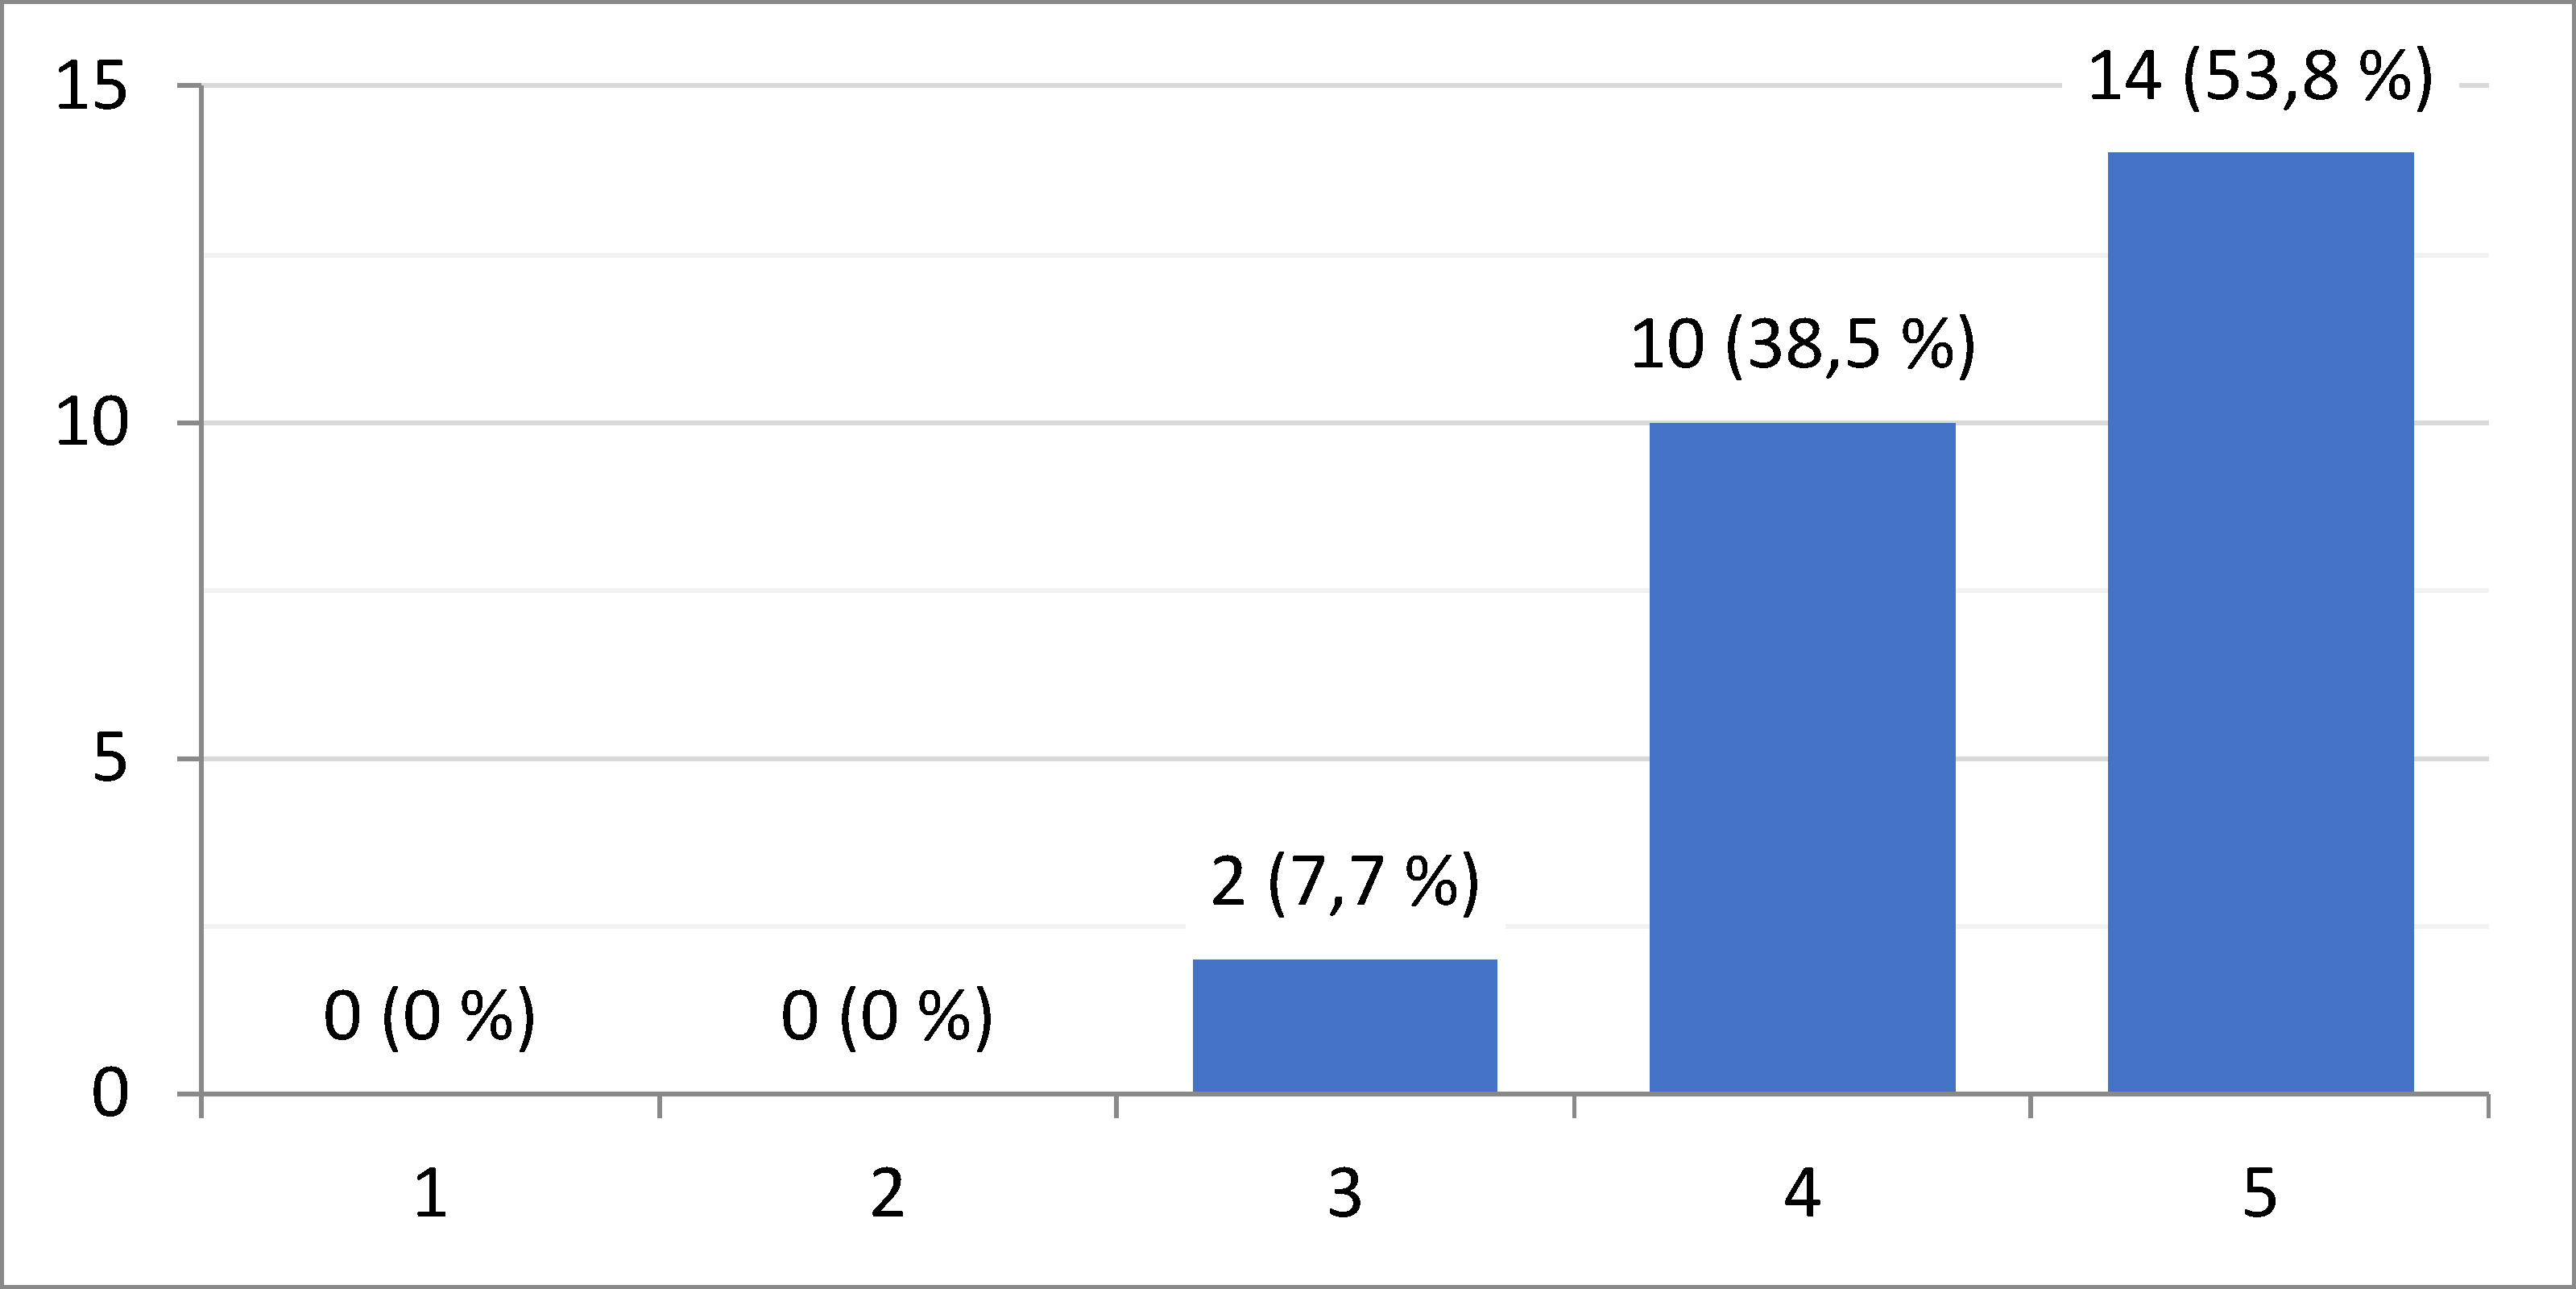
\includegraphics[width=0.8\linewidth]{obrazky-figures/graph1.pdf}
    \caption{Obrázek obsahuje graf odpovědí na otázku o~přehlednosti
    označení chyb na stupnici od 1 do 5, kde 1 představuje \uv{Zcela nepřehledné}
    a~5 představuje \uv{Jasné}.}
\end{figure}

\todo{další odpovědi}


%#######################    5.4 Možné budoucí rozšíření aplikace    #######################
\section{Možné budoucí rozšíření aplikace}
\todo{TODO: checkboxy pro nastavení kontrol, okraje pro oboustranný tisk, použití vektorových obrázků a ne rastrových, použití správných uvozovek, hledání nevhodných slov, jednopísmenné spojky na koci řádku,  proměnná \texttt{\_\_currPageTextContent} nebude obsahovat z embedded pdfs}

%*********************************************************************************




%*********************************************************************************
%                                   6 ZÁVĚR
%*********************************************************************************
\chapter{Závěr}
Cílem této bakalářské práce bylo vytvořit lehce dostupnou aplikaci, která zpracuje
nahraný PDF dokument a~pomocí PDF anotací v~něm vyznačí nalezené chyby. Tato
aplikace byla vytvořena jako webový nástroj a~nyní je veřejně
přístupná pod názvem Theses Checker\footnote{Theses Checker je dostupný na adrese
\href{https://theseschecker.eu.pythonanywhere.com/}{https://theseschecker.eu.pythonanywhere.com/}}.

Nejdříve bylo zapotřebí nalézt, které chyby se nejčastěji vyskytují v~závěrečných
pracích. Ty se nalezly zkoumáním zveřejněných textů a~posudků diplomových prací
vytvořených na Fakultě informačních technologií Vysokého učení technického v~Brně.
Poté byly zkoumány některé dostupné aplikace pro kontrolu textu. Bylo zjištěno,
že žádná dosavadní aplikace se nezaměřuje na typografickou stránku textu, jelikož
se většinou zaměřují na gramatiku.

Další na řadě bylo navrhnutí vzhledu aplikace a~označení nalezených chyb.
V~návrhu a~implementaci byla dána velká váha na přívětivost pro uživatele.
Aplikace se postupně měnila i~na základě zpětné vazby od uživatelů, která byla
podávána pomocí dotazníku.

Program umí kontrolovat šest typů chyb a~to přetečení za okraj stránky, 
špatné použití spojovníku, nevhodná šířka obrázku, vynechaná mezera před levou
závorkou, chybějící text mezi názvy sekcí a~odkaz na neexistující referenci.
Byl vytvořen plakát a~video\footnote{\todo{TODO: odkaz na video}} o~použití 
tohoto programu, čímž byl splněn poslední bod zadání této bakalářské práce.

Do budoucna bych chtěla vylepšit algoritmus na hledání okrajů PDF stránky
a~přidat pro něj podporu dokumentů nastavených na oboustranný tisk, jejichž
okraje jsou pro sudé a~liché stránky rozdílné. Dále bych chtěla vylepšit chování
kontrol pro textové objekty, jako jsou tabulky či výpisy.






%*********************************************************************************




%===============================================================================

% Pro kompilaci po částech (viz projekt.tex) nutno odkomentovat
%\end{document}
